% Options for packages loaded elsewhere
\PassOptionsToPackage{unicode}{hyperref}
\PassOptionsToPackage{hyphens}{url}
\PassOptionsToPackage{dvipsnames,svgnames,x11names}{xcolor}
%
\documentclass[
]{article}
\usepackage{amsmath,amssymb}
\usepackage{lmodern}
\usepackage{iftex}
\ifPDFTeX
  \usepackage[T1]{fontenc}
  \usepackage[utf8]{inputenc}
  \usepackage{textcomp} % provide euro and other symbols
\else % if luatex or xetex
  \usepackage{unicode-math}
  \defaultfontfeatures{Scale=MatchLowercase}
  \defaultfontfeatures[\rmfamily]{Ligatures=TeX,Scale=1}
\fi
% Use upquote if available, for straight quotes in verbatim environments
\IfFileExists{upquote.sty}{\usepackage{upquote}}{}
\IfFileExists{microtype.sty}{% use microtype if available
  \usepackage[]{microtype}
  \UseMicrotypeSet[protrusion]{basicmath} % disable protrusion for tt fonts
}{}
\makeatletter
\@ifundefined{KOMAClassName}{% if non-KOMA class
  \IfFileExists{parskip.sty}{%
    \usepackage{parskip}
  }{% else
    \setlength{\parindent}{0pt}
    \setlength{\parskip}{6pt plus 2pt minus 1pt}}
}{% if KOMA class
  \KOMAoptions{parskip=half}}
\makeatother
\usepackage{xcolor}
\usepackage[margin=1in]{geometry}
\usepackage{color}
\usepackage{fancyvrb}
\newcommand{\VerbBar}{|}
\newcommand{\VERB}{\Verb[commandchars=\\\{\}]}
\DefineVerbatimEnvironment{Highlighting}{Verbatim}{commandchars=\\\{\}}
% Add ',fontsize=\small' for more characters per line
\usepackage{framed}
\definecolor{shadecolor}{RGB}{248,248,248}
\newenvironment{Shaded}{\begin{snugshade}}{\end{snugshade}}
\newcommand{\AlertTok}[1]{\textcolor[rgb]{0.94,0.16,0.16}{#1}}
\newcommand{\AnnotationTok}[1]{\textcolor[rgb]{0.56,0.35,0.01}{\textbf{\textit{#1}}}}
\newcommand{\AttributeTok}[1]{\textcolor[rgb]{0.77,0.63,0.00}{#1}}
\newcommand{\BaseNTok}[1]{\textcolor[rgb]{0.00,0.00,0.81}{#1}}
\newcommand{\BuiltInTok}[1]{#1}
\newcommand{\CharTok}[1]{\textcolor[rgb]{0.31,0.60,0.02}{#1}}
\newcommand{\CommentTok}[1]{\textcolor[rgb]{0.56,0.35,0.01}{\textit{#1}}}
\newcommand{\CommentVarTok}[1]{\textcolor[rgb]{0.56,0.35,0.01}{\textbf{\textit{#1}}}}
\newcommand{\ConstantTok}[1]{\textcolor[rgb]{0.00,0.00,0.00}{#1}}
\newcommand{\ControlFlowTok}[1]{\textcolor[rgb]{0.13,0.29,0.53}{\textbf{#1}}}
\newcommand{\DataTypeTok}[1]{\textcolor[rgb]{0.13,0.29,0.53}{#1}}
\newcommand{\DecValTok}[1]{\textcolor[rgb]{0.00,0.00,0.81}{#1}}
\newcommand{\DocumentationTok}[1]{\textcolor[rgb]{0.56,0.35,0.01}{\textbf{\textit{#1}}}}
\newcommand{\ErrorTok}[1]{\textcolor[rgb]{0.64,0.00,0.00}{\textbf{#1}}}
\newcommand{\ExtensionTok}[1]{#1}
\newcommand{\FloatTok}[1]{\textcolor[rgb]{0.00,0.00,0.81}{#1}}
\newcommand{\FunctionTok}[1]{\textcolor[rgb]{0.00,0.00,0.00}{#1}}
\newcommand{\ImportTok}[1]{#1}
\newcommand{\InformationTok}[1]{\textcolor[rgb]{0.56,0.35,0.01}{\textbf{\textit{#1}}}}
\newcommand{\KeywordTok}[1]{\textcolor[rgb]{0.13,0.29,0.53}{\textbf{#1}}}
\newcommand{\NormalTok}[1]{#1}
\newcommand{\OperatorTok}[1]{\textcolor[rgb]{0.81,0.36,0.00}{\textbf{#1}}}
\newcommand{\OtherTok}[1]{\textcolor[rgb]{0.56,0.35,0.01}{#1}}
\newcommand{\PreprocessorTok}[1]{\textcolor[rgb]{0.56,0.35,0.01}{\textit{#1}}}
\newcommand{\RegionMarkerTok}[1]{#1}
\newcommand{\SpecialCharTok}[1]{\textcolor[rgb]{0.00,0.00,0.00}{#1}}
\newcommand{\SpecialStringTok}[1]{\textcolor[rgb]{0.31,0.60,0.02}{#1}}
\newcommand{\StringTok}[1]{\textcolor[rgb]{0.31,0.60,0.02}{#1}}
\newcommand{\VariableTok}[1]{\textcolor[rgb]{0.00,0.00,0.00}{#1}}
\newcommand{\VerbatimStringTok}[1]{\textcolor[rgb]{0.31,0.60,0.02}{#1}}
\newcommand{\WarningTok}[1]{\textcolor[rgb]{0.56,0.35,0.01}{\textbf{\textit{#1}}}}
\usepackage{graphicx}
\makeatletter
\def\maxwidth{\ifdim\Gin@nat@width>\linewidth\linewidth\else\Gin@nat@width\fi}
\def\maxheight{\ifdim\Gin@nat@height>\textheight\textheight\else\Gin@nat@height\fi}
\makeatother
% Scale images if necessary, so that they will not overflow the page
% margins by default, and it is still possible to overwrite the defaults
% using explicit options in \includegraphics[width, height, ...]{}
\setkeys{Gin}{width=\maxwidth,height=\maxheight,keepaspectratio}
% Set default figure placement to htbp
\makeatletter
\def\fps@figure{htbp}
\makeatother
\setlength{\emergencystretch}{3em} % prevent overfull lines
\providecommand{\tightlist}{%
  \setlength{\itemsep}{0pt}\setlength{\parskip}{0pt}}
\setcounter{secnumdepth}{5}
\newlength{\cslhangindent}
\setlength{\cslhangindent}{1.5em}
\newlength{\csllabelwidth}
\setlength{\csllabelwidth}{3em}
\newlength{\cslentryspacingunit} % times entry-spacing
\setlength{\cslentryspacingunit}{\parskip}
\newenvironment{CSLReferences}[2] % #1 hanging-ident, #2 entry spacing
 {% don't indent paragraphs
  \setlength{\parindent}{0pt}
  % turn on hanging indent if param 1 is 1
  \ifodd #1
  \let\oldpar\par
  \def\par{\hangindent=\cslhangindent\oldpar}
  \fi
  % set entry spacing
  \setlength{\parskip}{#2\cslentryspacingunit}
 }%
 {}
\usepackage{calc}
\newcommand{\CSLBlock}[1]{#1\hfill\break}
\newcommand{\CSLLeftMargin}[1]{\parbox[t]{\csllabelwidth}{#1}}
\newcommand{\CSLRightInline}[1]{\parbox[t]{\linewidth - \csllabelwidth}{#1}\break}
\newcommand{\CSLIndent}[1]{\hspace{\cslhangindent}#1}
\ifLuaTeX
  \usepackage{selnolig}  % disable illegal ligatures
\fi
\IfFileExists{bookmark.sty}{\usepackage{bookmark}}{\usepackage{hyperref}}
\IfFileExists{xurl.sty}{\usepackage{xurl}}{} % add URL line breaks if available
\urlstyle{same} % disable monospaced font for URLs
\hypersetup{
  pdftitle={Respiratory Rate Determination by Non-Invasive Means},
  pdfauthor={Stephen Su, 844503, COMP90072},
  colorlinks=true,
  linkcolor={Maroon},
  filecolor={Maroon},
  citecolor={Blue},
  urlcolor={blue},
  pdfcreator={LaTeX via pandoc}}

\title{Respiratory Rate Determination by Non-Invasive Means}
\author{Stephen Su, 844503, COMP90072}
\date{}

\begin{document}
\maketitle

\hypertarget{introduction}{%
\section{Introduction}\label{introduction}}

\hypertarget{background}{%
\subsection{Background}\label{background}}

(Penzel et al., 2000).

\hypertarget{the-data}{%
\section{The data}\label{the-data}}

\hypertarget{data-source}{%
\subsection{Data source}\label{data-source}}

(Goldberger et al., 2000).

\hypertarget{sample-plot}{%
\subsection{Sample plot}\label{sample-plot}}

\begin{center}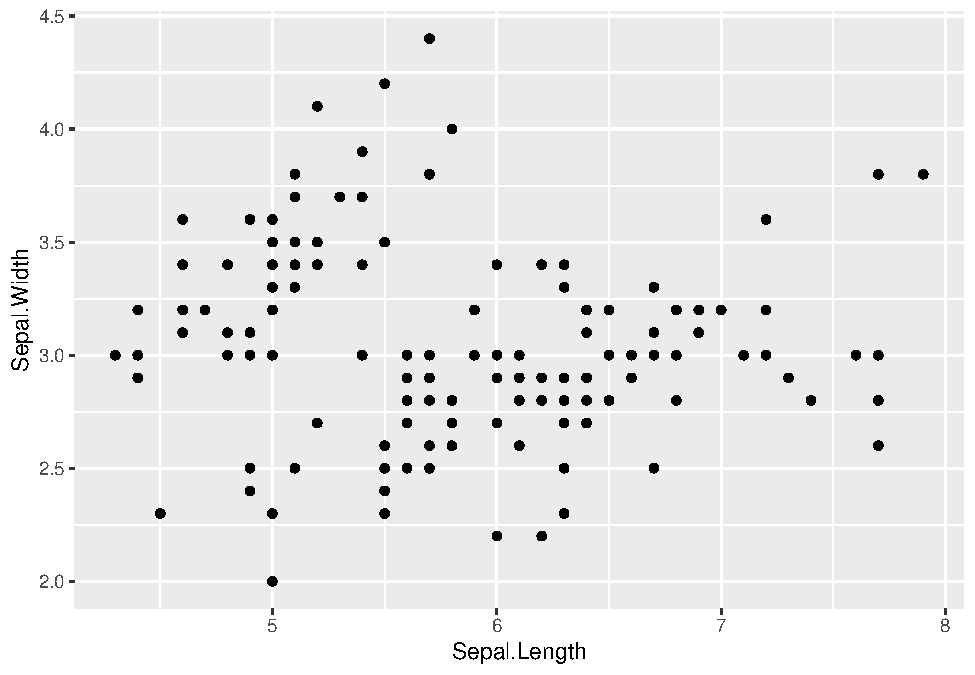
\includegraphics{report_files/figure-latex/data-1} \end{center}

\begin{center}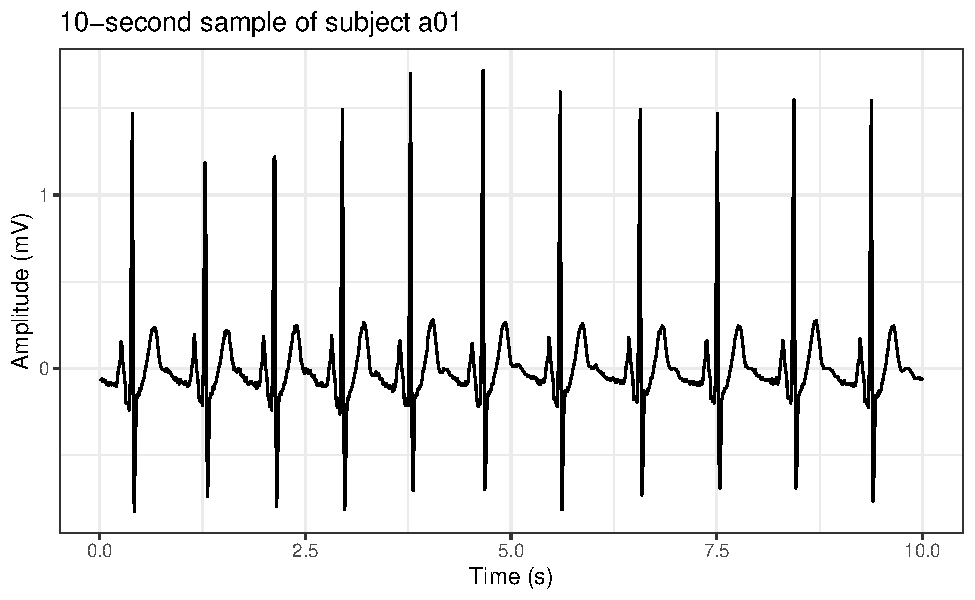
\includegraphics{report_files/figure-latex/rr-interval-1} \end{center}

\begin{Shaded}
\begin{Highlighting}[]
\NormalTok{interval }\OtherTok{\textless{}{-}} \FunctionTok{rr\_interval}\NormalTok{(data}\SpecialCharTok{$}\NormalTok{voltage)}
\FunctionTok{range}\NormalTok{(interval) }\DocumentationTok{\#\# Range of R{-}R intervals}
\end{Highlighting}
\end{Shaded}

\begin{verbatim}
#> [1] 0.13 1.89
\end{verbatim}

\begin{Shaded}
\begin{Highlighting}[]
\DecValTok{60} \SpecialCharTok{/} \FunctionTok{range}\NormalTok{(interval) }\DocumentationTok{\#\# Range of instantaneous heart rate per minute}
\end{Highlighting}
\end{Shaded}

\begin{verbatim}
#> [1] 461.53846  31.74603
\end{verbatim}

\begin{Shaded}
\begin{Highlighting}[]
\NormalTok{abnormal\_interval }\OtherTok{\textless{}{-}} \FunctionTok{abnormal\_rr}\NormalTok{(data}\SpecialCharTok{$}\NormalTok{voltage, }\AttributeTok{max\_bpm =} \DecValTok{130}\NormalTok{, }\AttributeTok{min\_bpm =} \DecValTok{40}\NormalTok{)}
\FunctionTok{length}\NormalTok{(abnormal\_interval) }\DocumentationTok{\#\# Number of abnormal R{-}R intervals}
\end{Highlighting}
\end{Shaded}

\begin{verbatim}
#> [1] 58
\end{verbatim}

\begin{Shaded}
\begin{Highlighting}[]
\FunctionTok{length}\NormalTok{(interval) }\DocumentationTok{\#\# Total number of heart beats}
\end{Highlighting}
\end{Shaded}

\begin{verbatim}
#> [1] 29941
\end{verbatim}

\begin{Shaded}
\begin{Highlighting}[]
\FunctionTok{invisible}\NormalTok{(}\FunctionTok{map}\NormalTok{(}\FunctionTok{seq\_len}\NormalTok{(}\DecValTok{58}\NormalTok{), }\ControlFlowTok{function}\NormalTok{(i) }\FunctionTok{print}\NormalTok{(}\FunctionTok{plot\_abnormal\_rr}\NormalTok{(data, i))))}
\end{Highlighting}
\end{Shaded}

\begin{center}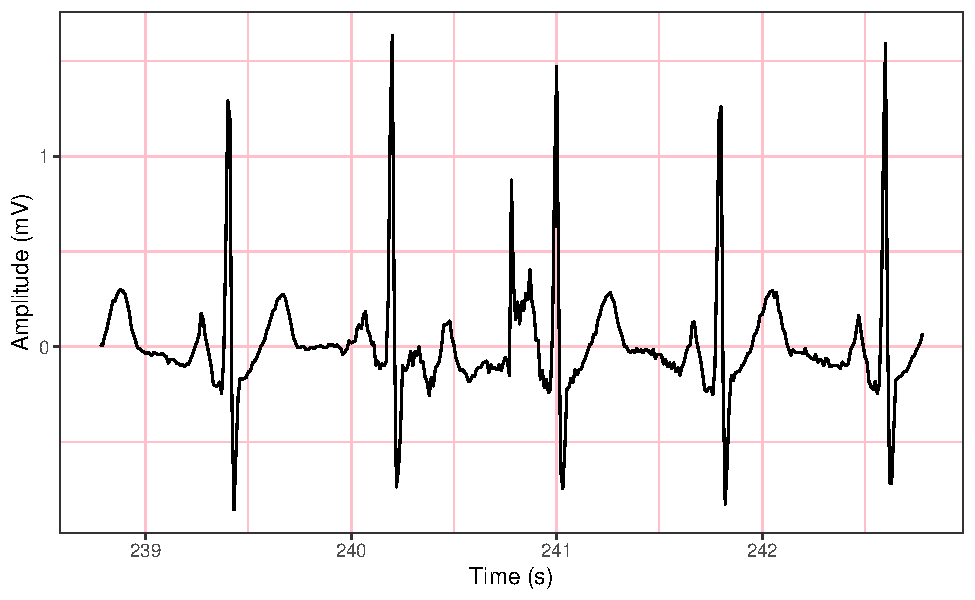
\includegraphics{report_files/figure-latex/abnormal-interval-1} \end{center}

\begin{center}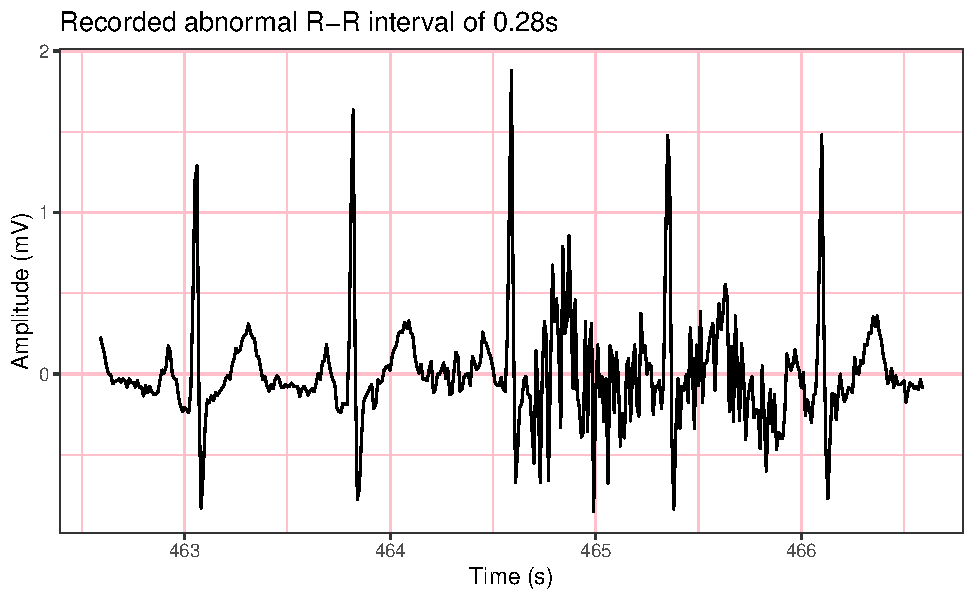
\includegraphics{report_files/figure-latex/abnormal-interval-2} \end{center}

\begin{center}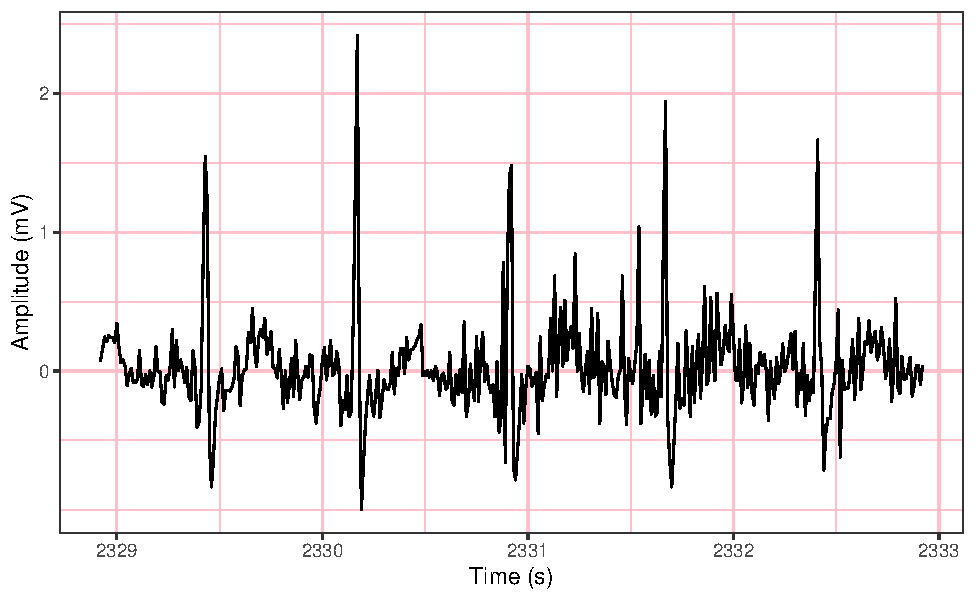
\includegraphics{report_files/figure-latex/abnormal-interval-3} \end{center}

\begin{center}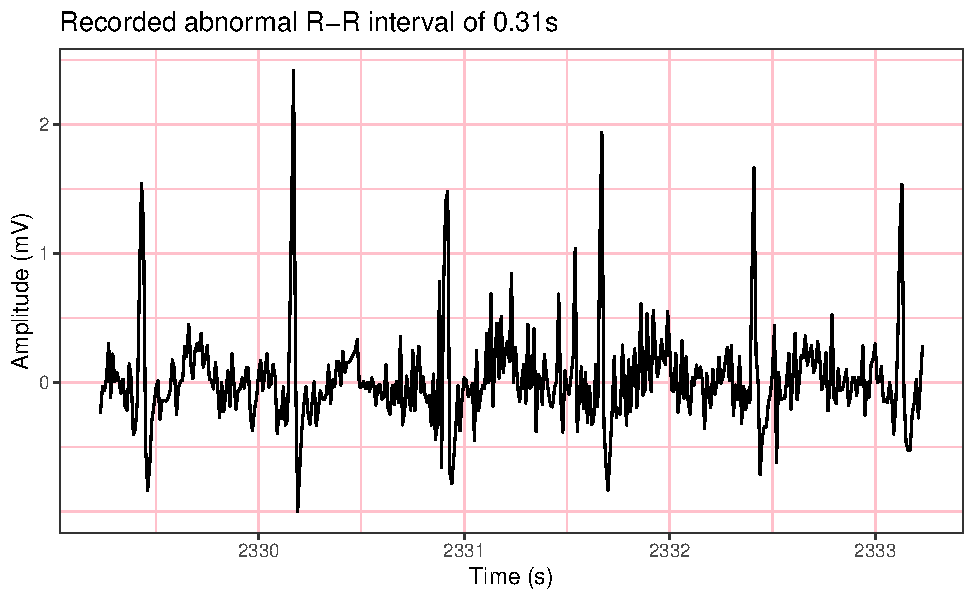
\includegraphics{report_files/figure-latex/abnormal-interval-4} \end{center}

\begin{center}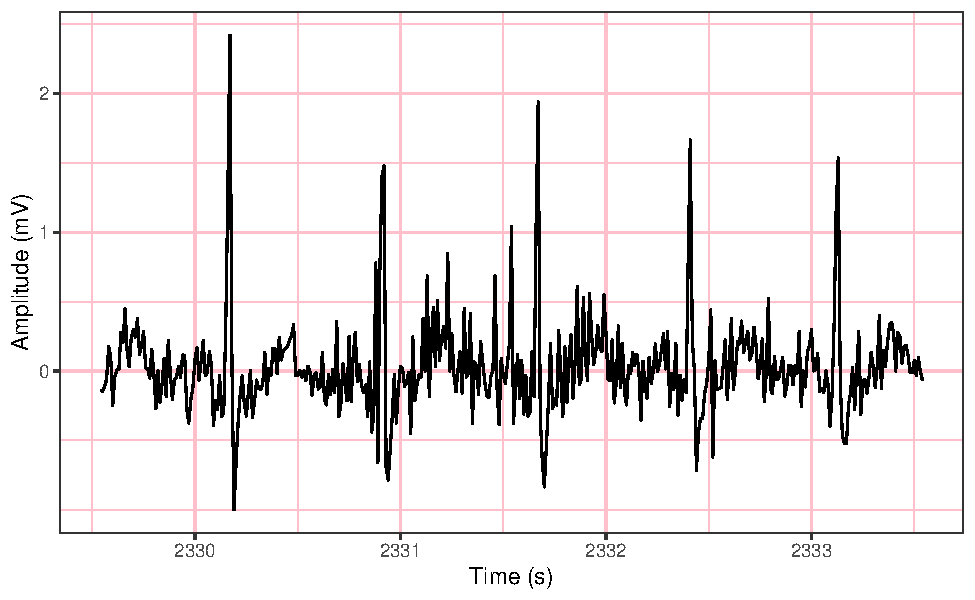
\includegraphics{report_files/figure-latex/abnormal-interval-5} \end{center}

\begin{center}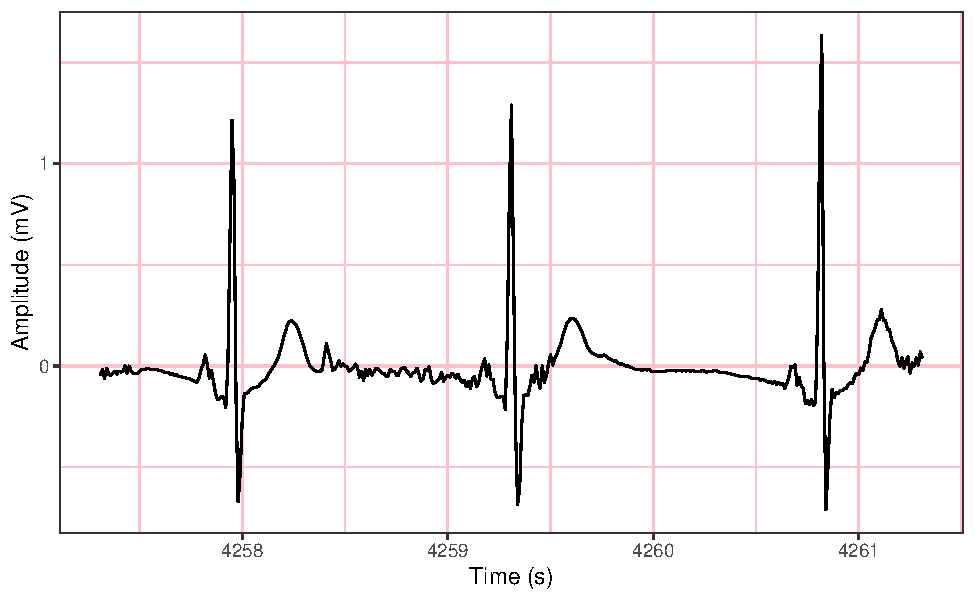
\includegraphics{report_files/figure-latex/abnormal-interval-6} \end{center}

\begin{center}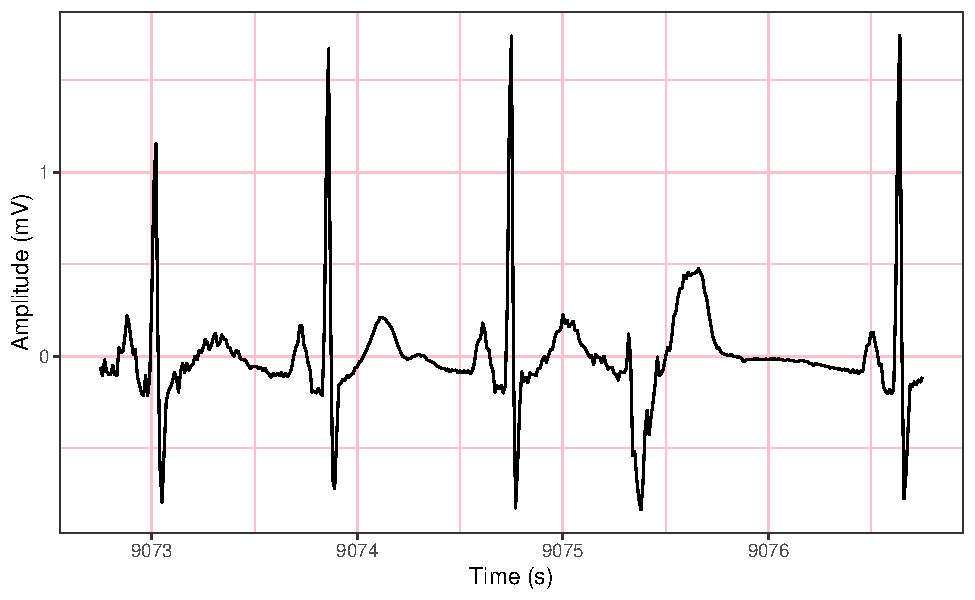
\includegraphics{report_files/figure-latex/abnormal-interval-7} \end{center}

\begin{center}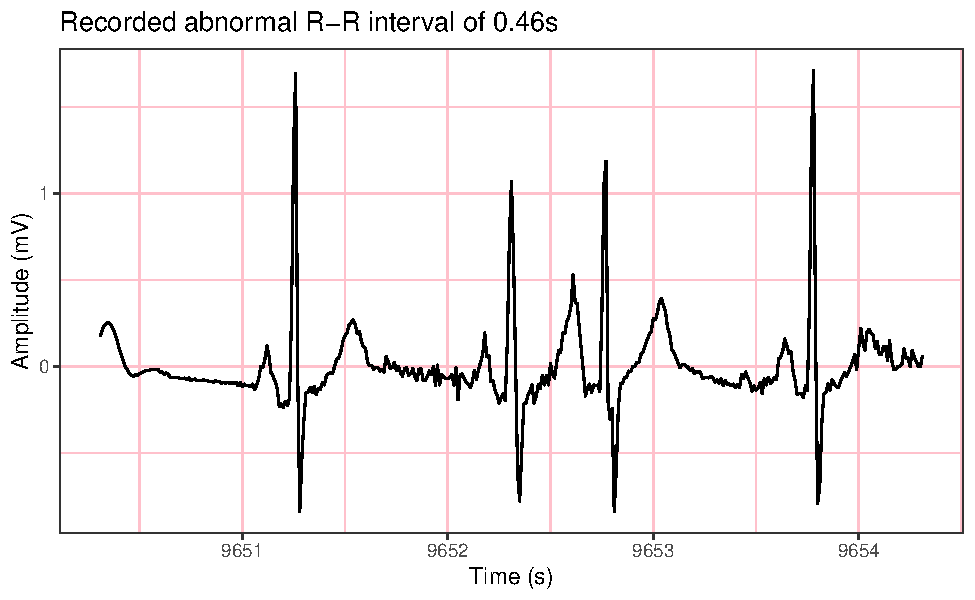
\includegraphics{report_files/figure-latex/abnormal-interval-8} \end{center}

\begin{center}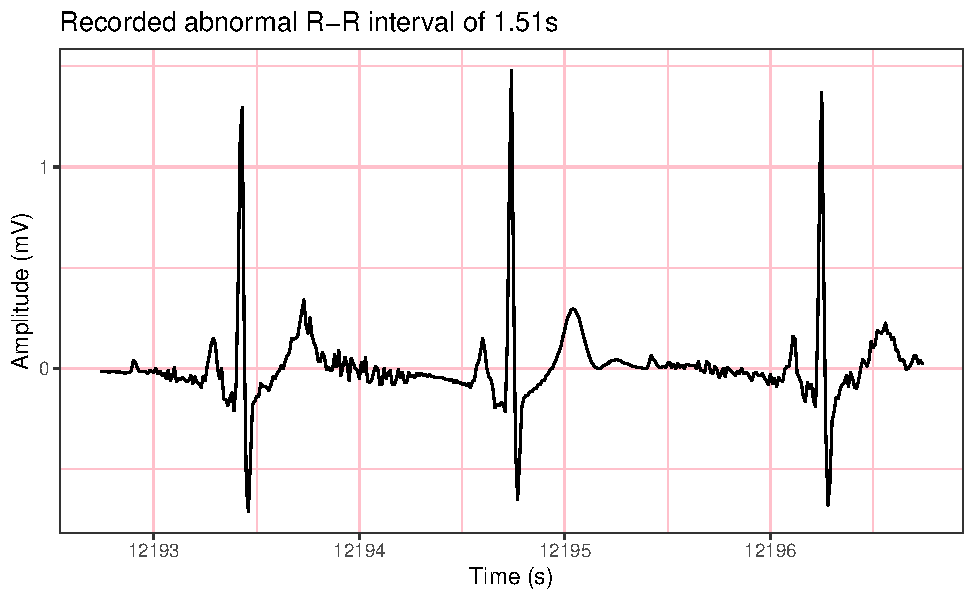
\includegraphics{report_files/figure-latex/abnormal-interval-9} \end{center}

\begin{center}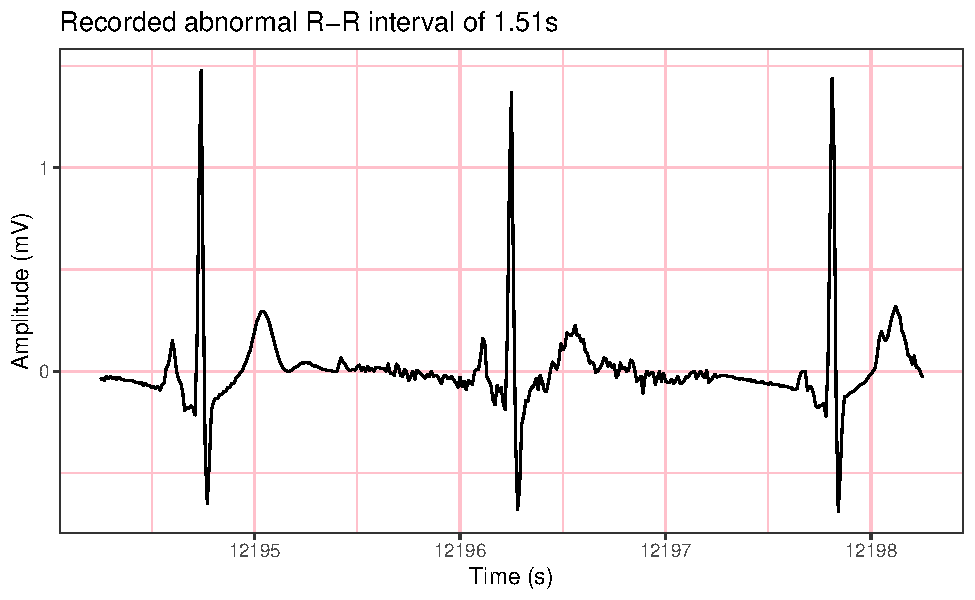
\includegraphics{report_files/figure-latex/abnormal-interval-10} \end{center}

\begin{center}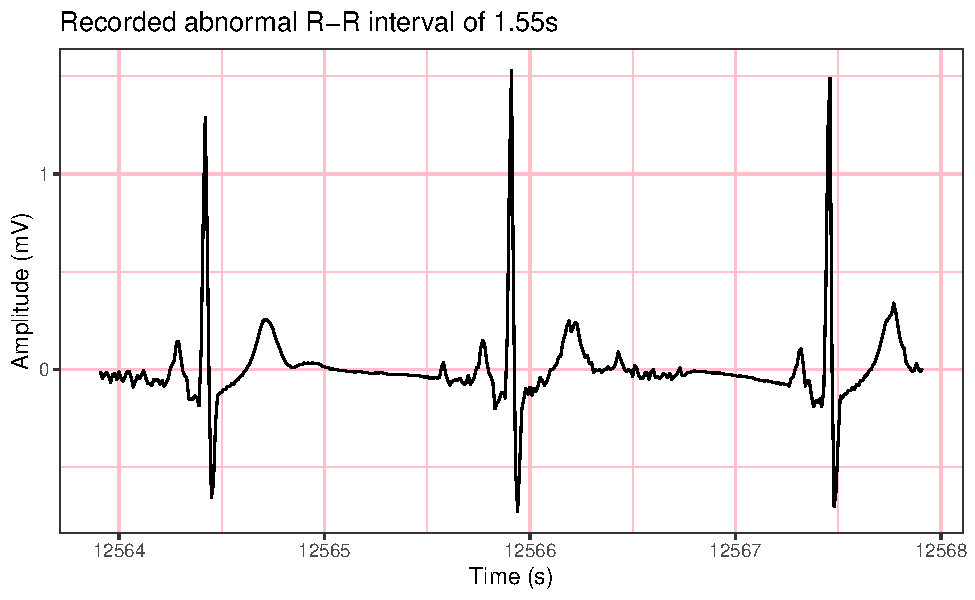
\includegraphics{report_files/figure-latex/abnormal-interval-11} \end{center}

\begin{center}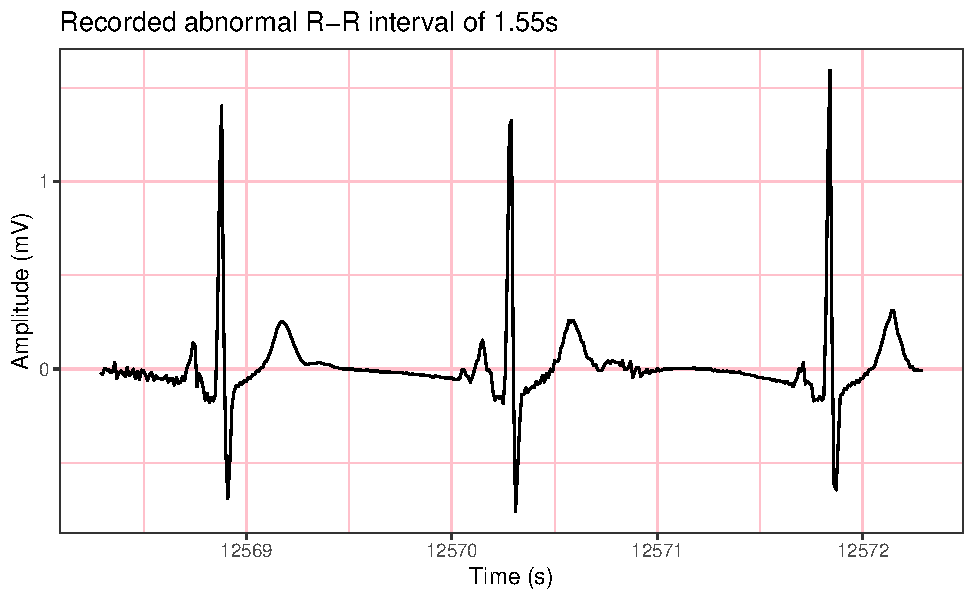
\includegraphics{report_files/figure-latex/abnormal-interval-12} \end{center}

\begin{center}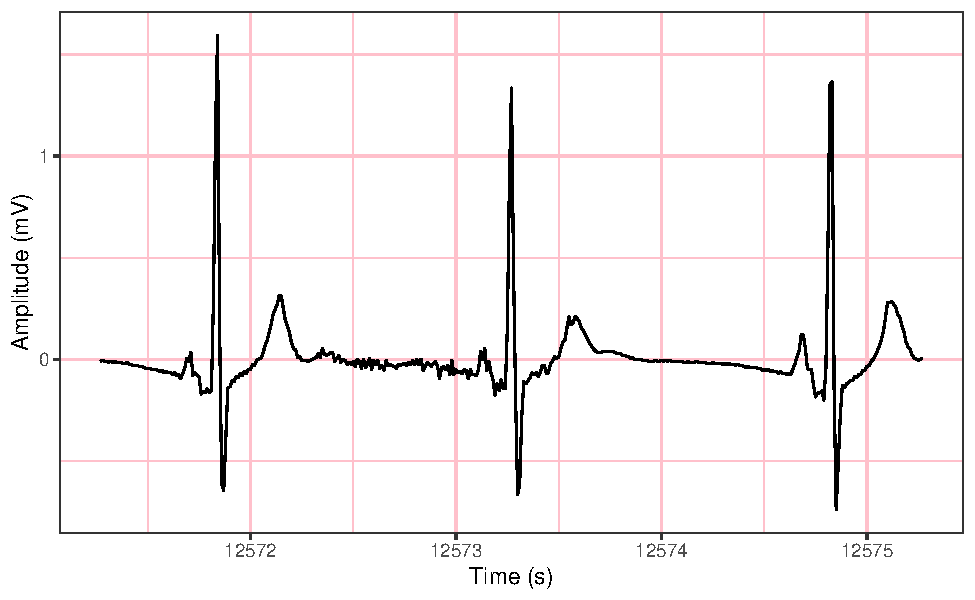
\includegraphics{report_files/figure-latex/abnormal-interval-13} \end{center}

\begin{center}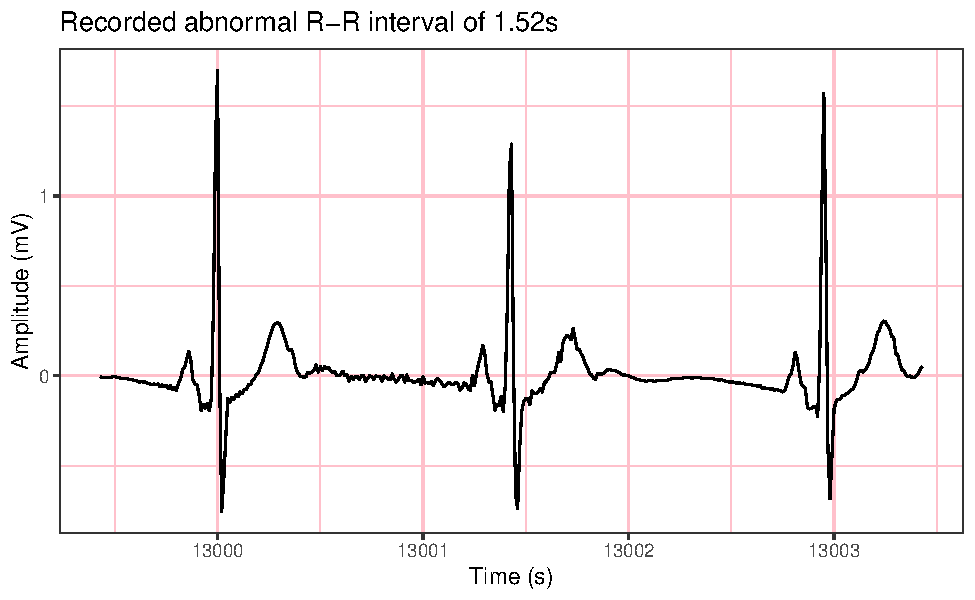
\includegraphics{report_files/figure-latex/abnormal-interval-14} \end{center}

\begin{center}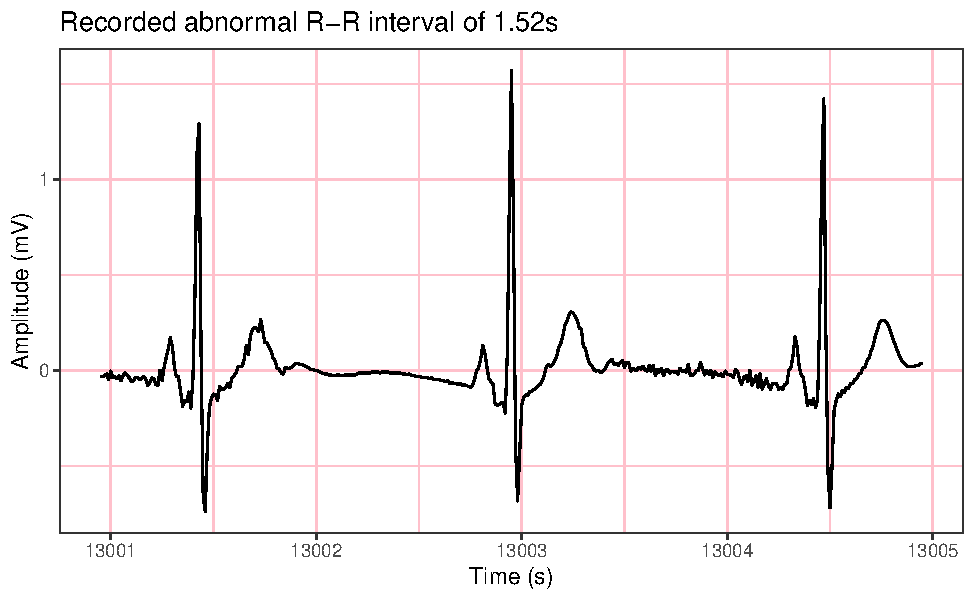
\includegraphics{report_files/figure-latex/abnormal-interval-15} \end{center}

\begin{center}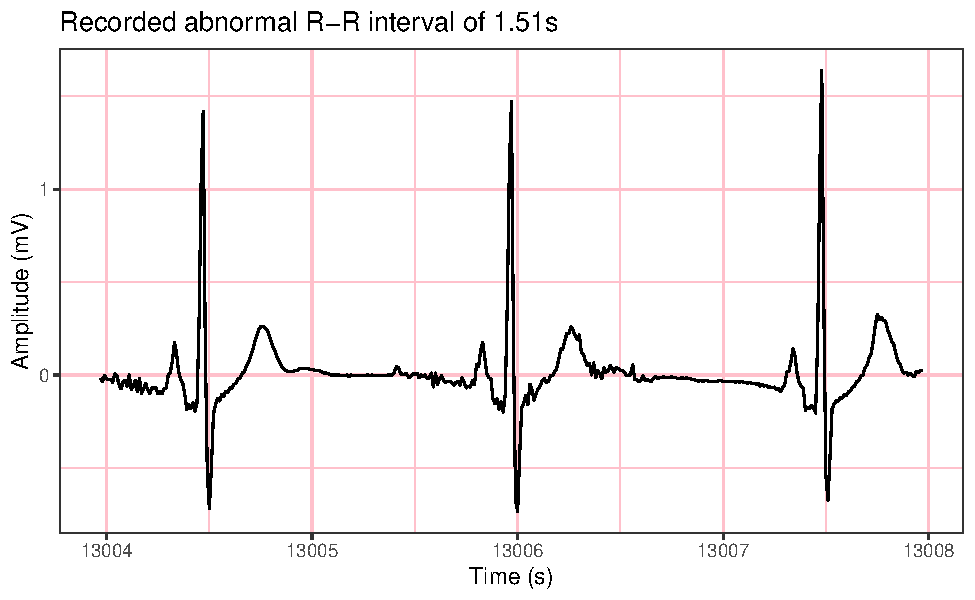
\includegraphics{report_files/figure-latex/abnormal-interval-16} \end{center}

\begin{center}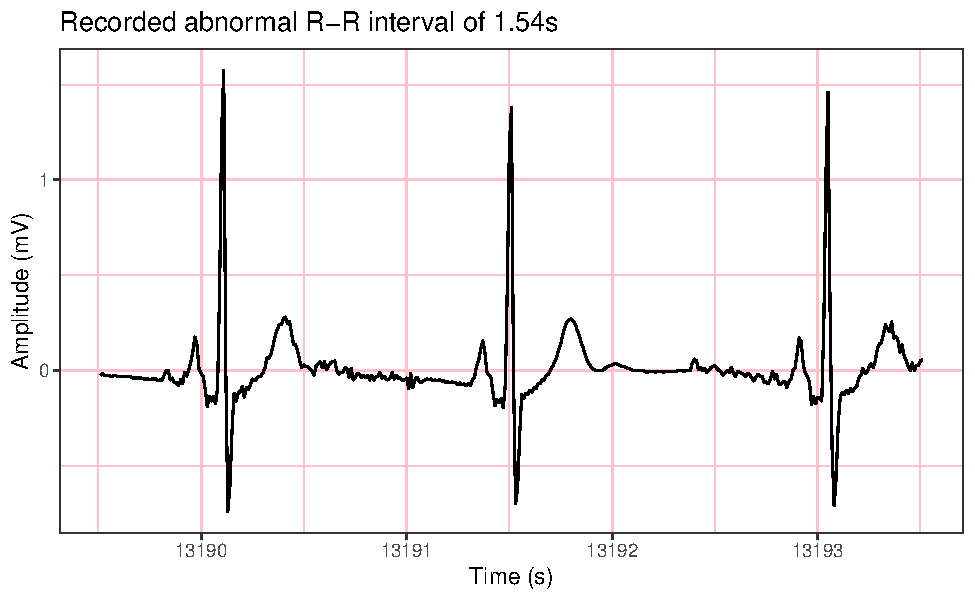
\includegraphics{report_files/figure-latex/abnormal-interval-17} \end{center}

\begin{center}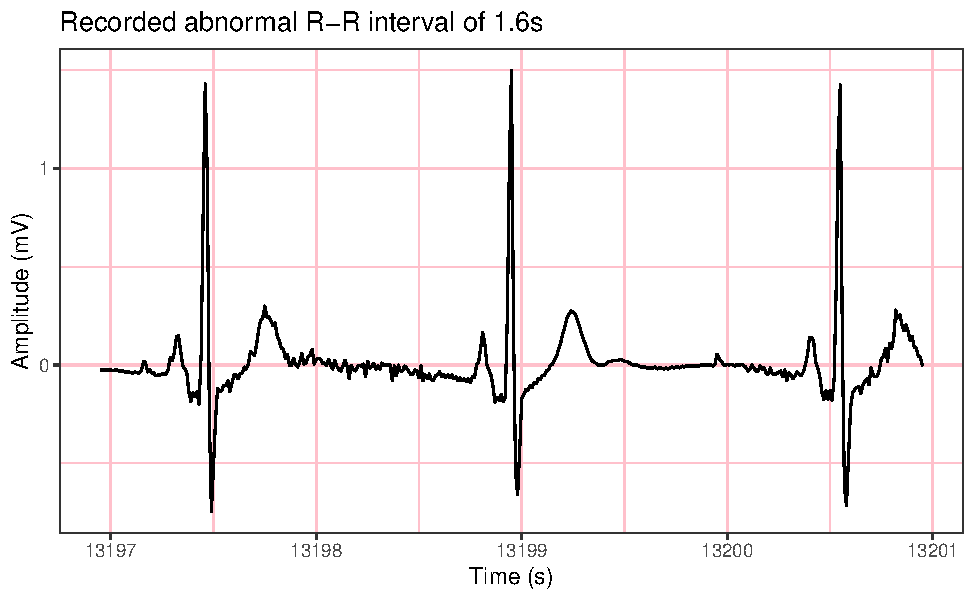
\includegraphics{report_files/figure-latex/abnormal-interval-18} \end{center}

\begin{center}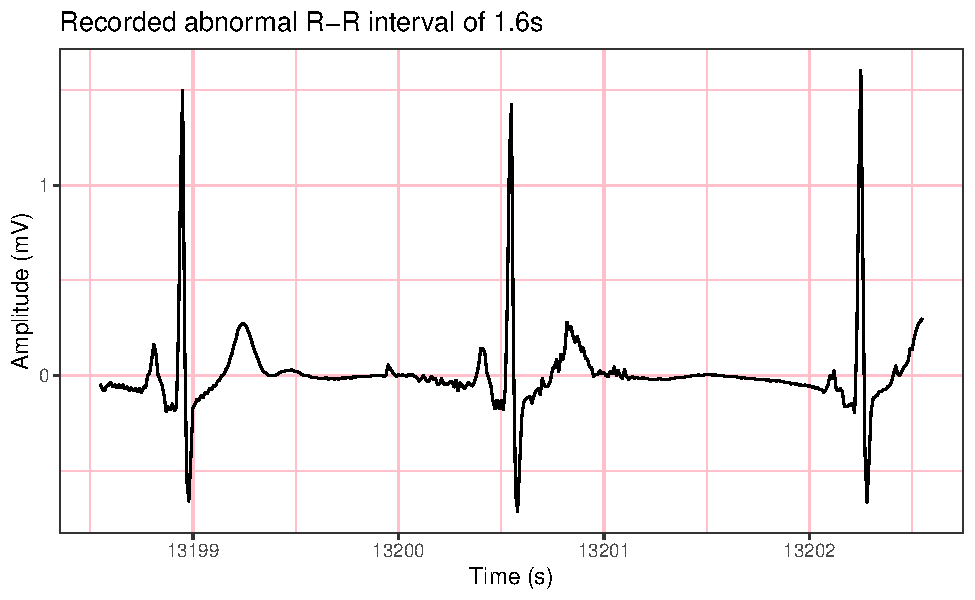
\includegraphics{report_files/figure-latex/abnormal-interval-19} \end{center}

\begin{center}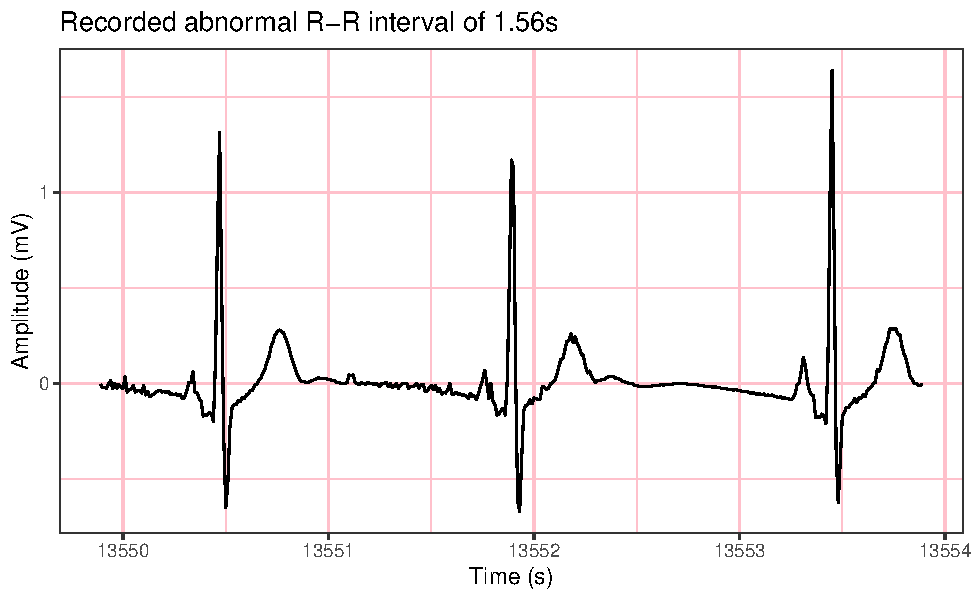
\includegraphics{report_files/figure-latex/abnormal-interval-20} \end{center}

\begin{center}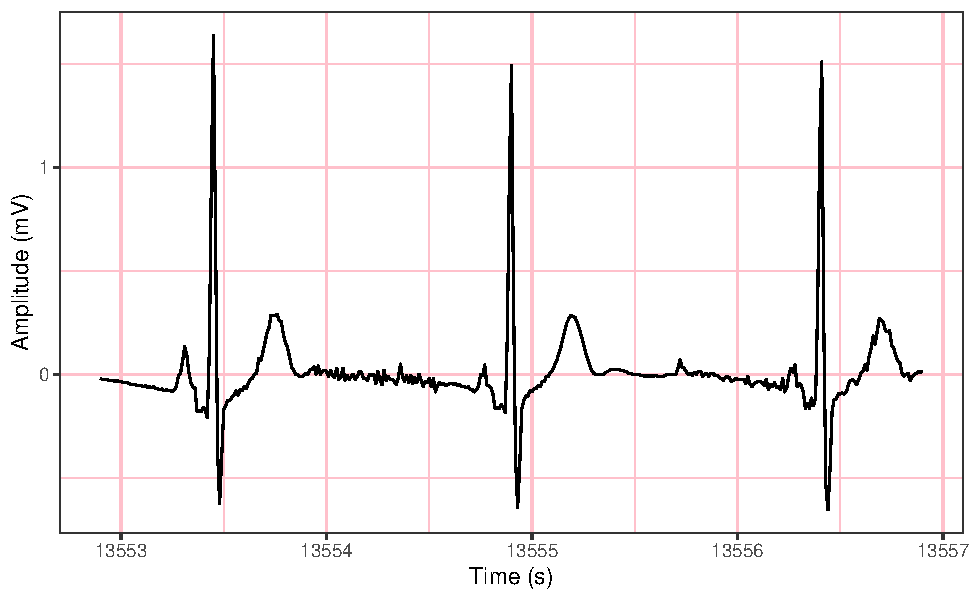
\includegraphics{report_files/figure-latex/abnormal-interval-21} \end{center}

\begin{center}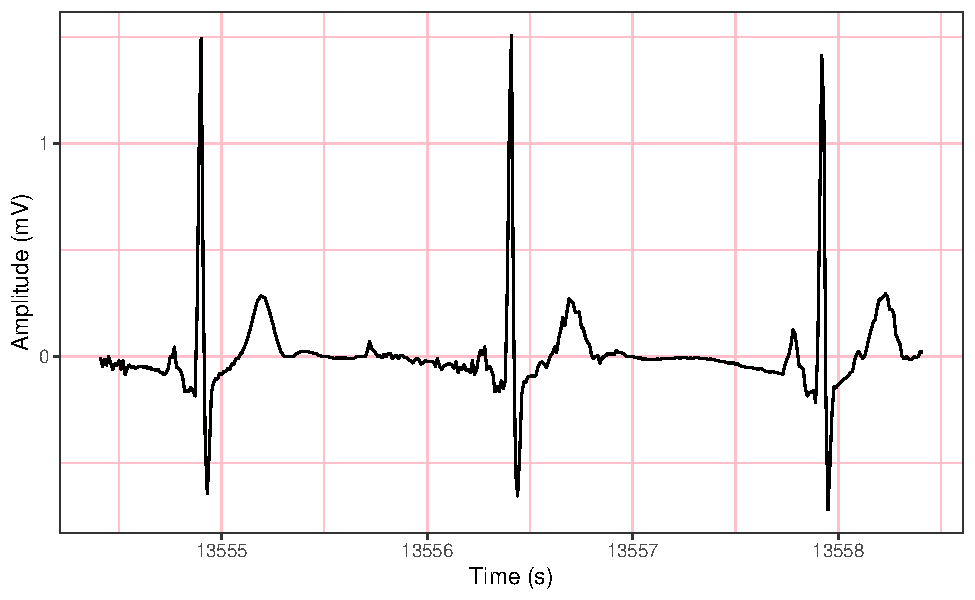
\includegraphics{report_files/figure-latex/abnormal-interval-22} \end{center}

\begin{center}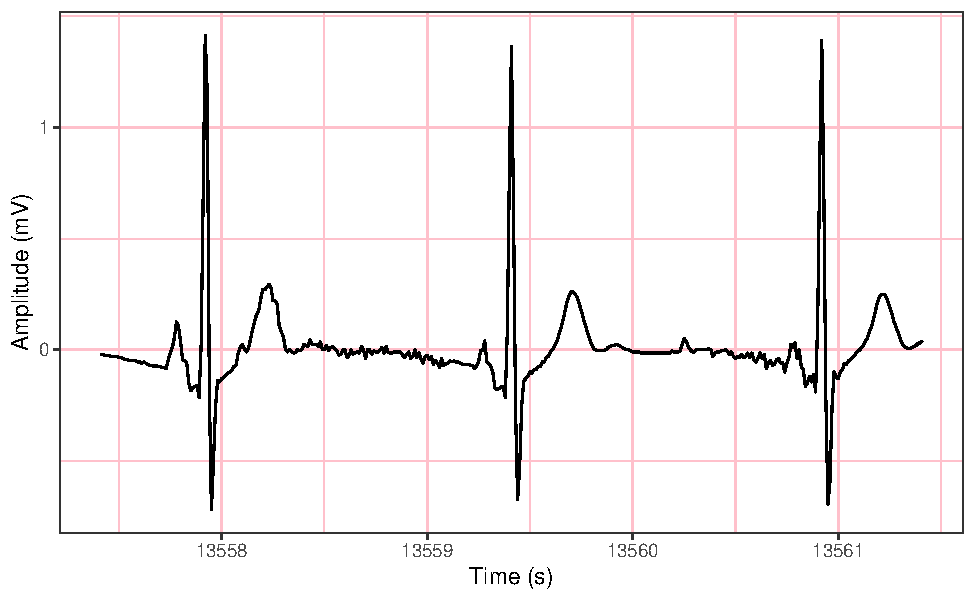
\includegraphics{report_files/figure-latex/abnormal-interval-23} \end{center}

\begin{center}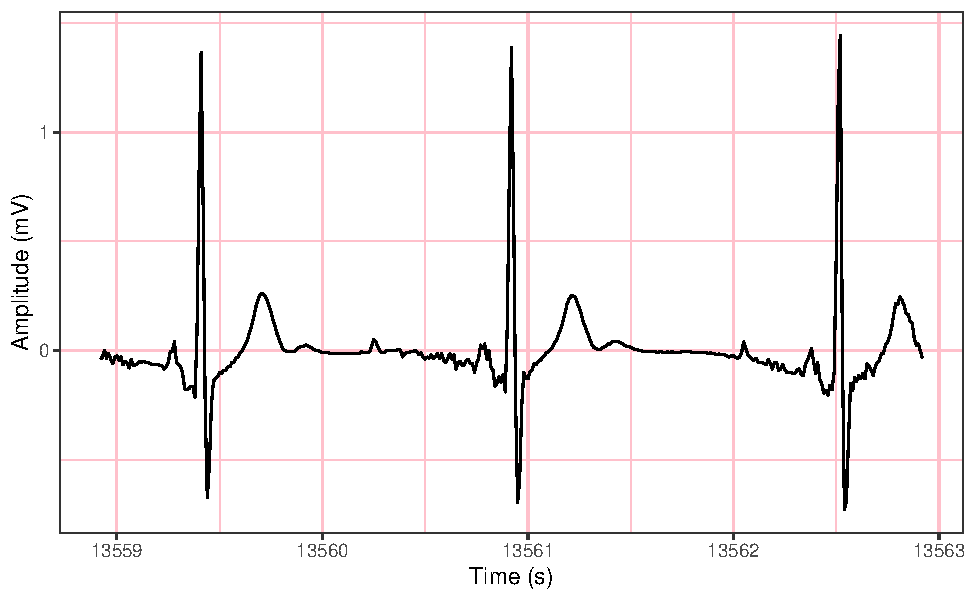
\includegraphics{report_files/figure-latex/abnormal-interval-24} \end{center}

\begin{center}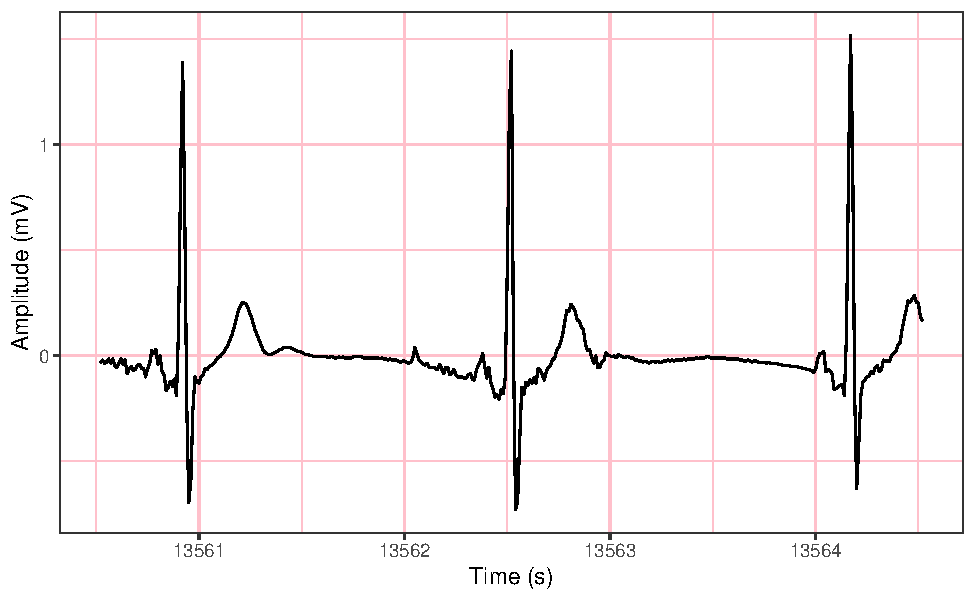
\includegraphics{report_files/figure-latex/abnormal-interval-25} \end{center}

\begin{center}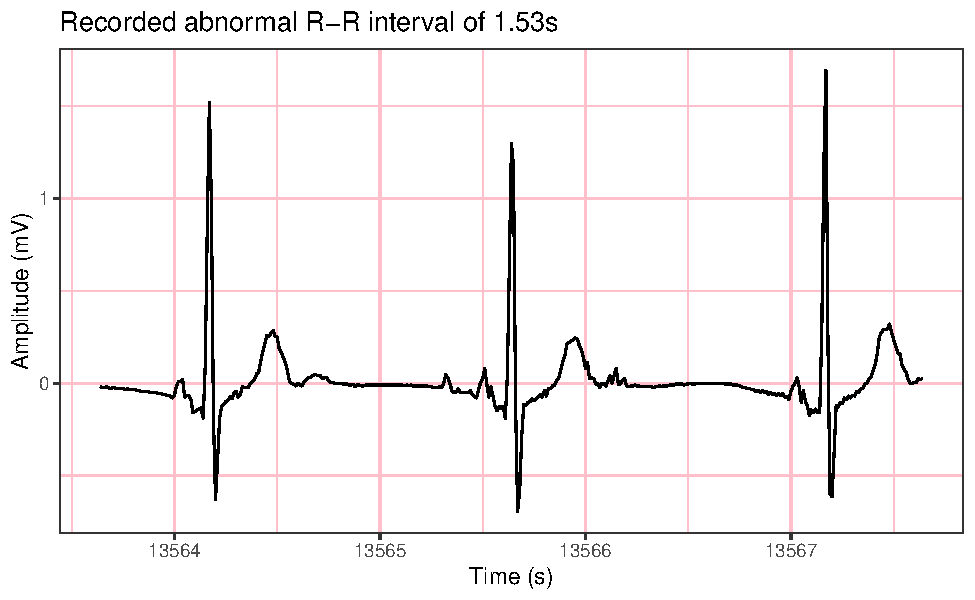
\includegraphics{report_files/figure-latex/abnormal-interval-26} \end{center}

\begin{center}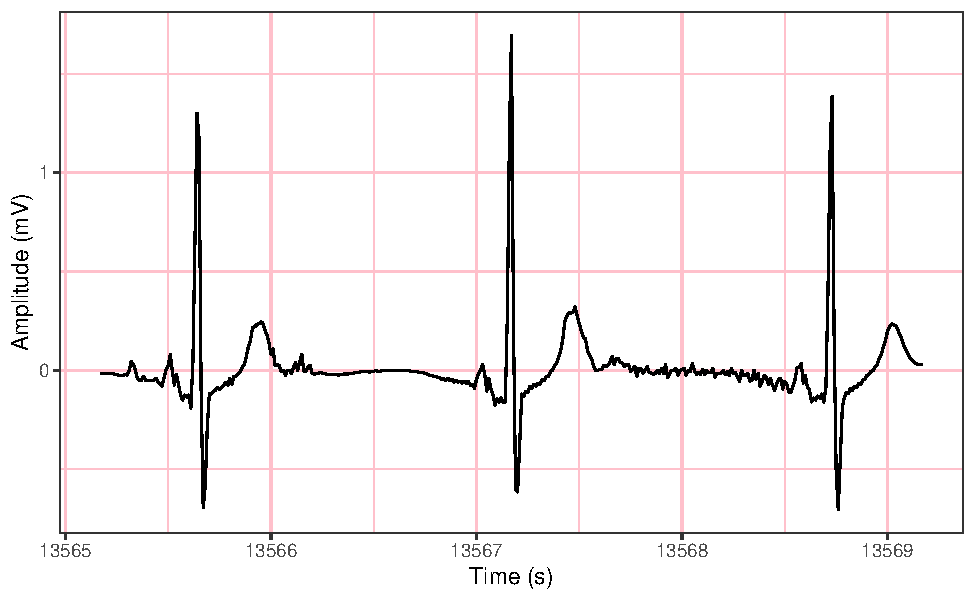
\includegraphics{report_files/figure-latex/abnormal-interval-27} \end{center}

\begin{center}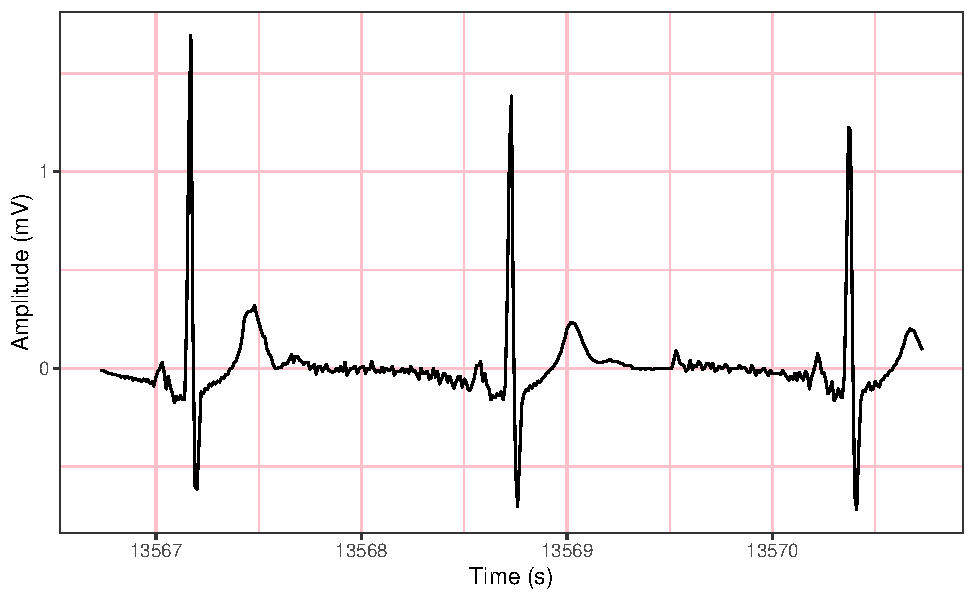
\includegraphics{report_files/figure-latex/abnormal-interval-28} \end{center}

\begin{center}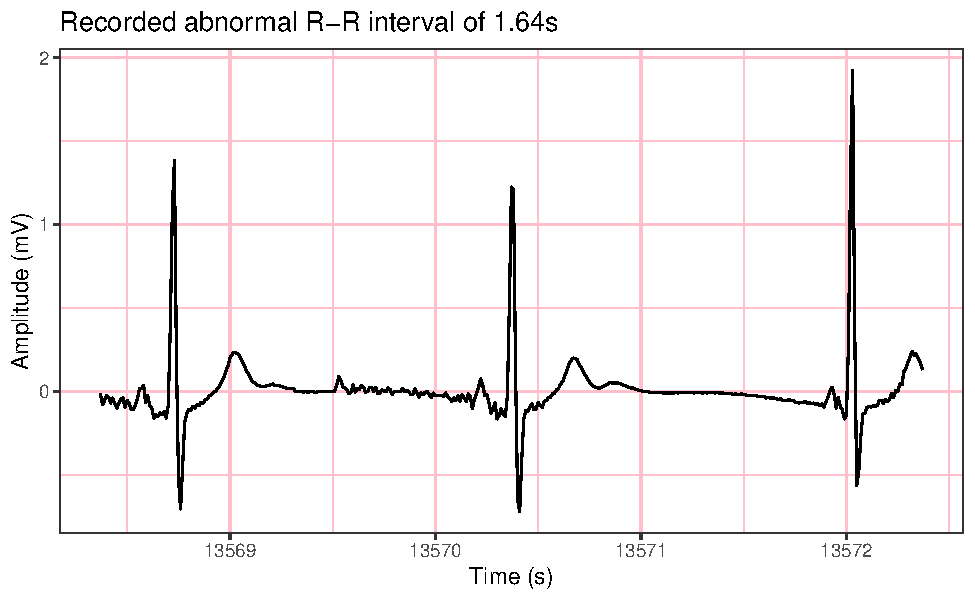
\includegraphics{report_files/figure-latex/abnormal-interval-29} \end{center}

\begin{center}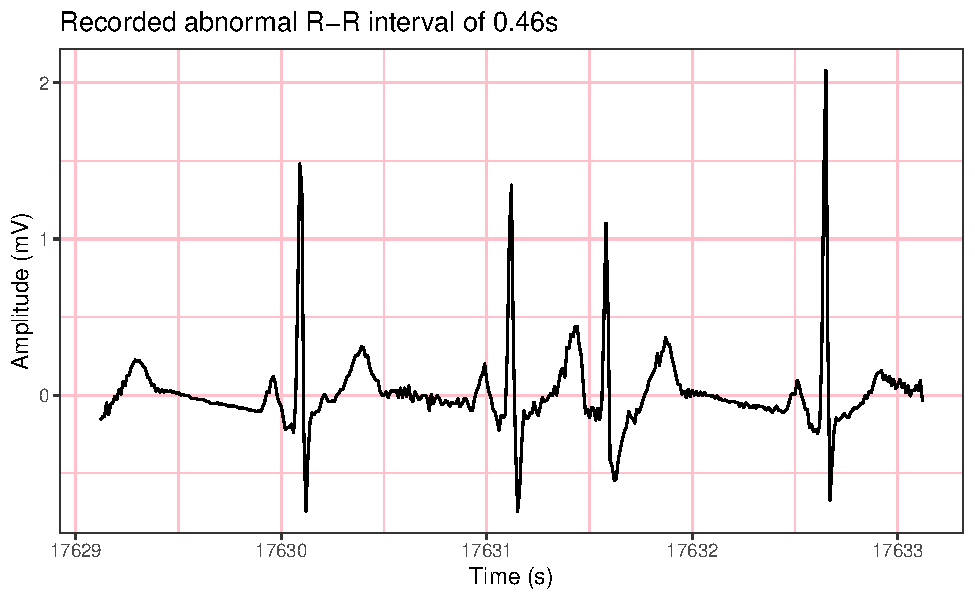
\includegraphics{report_files/figure-latex/abnormal-interval-30} \end{center}

\begin{center}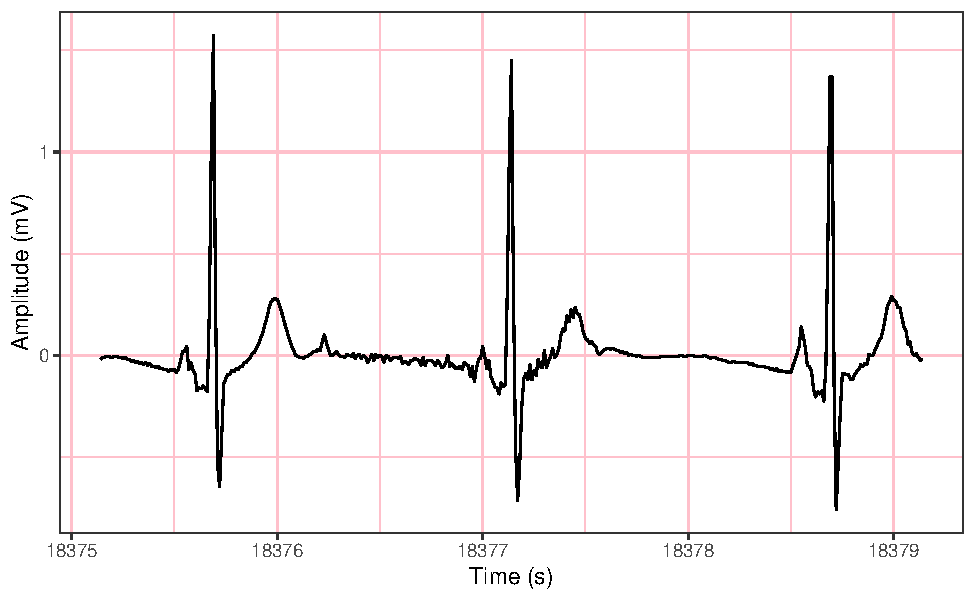
\includegraphics{report_files/figure-latex/abnormal-interval-31} \end{center}

\begin{center}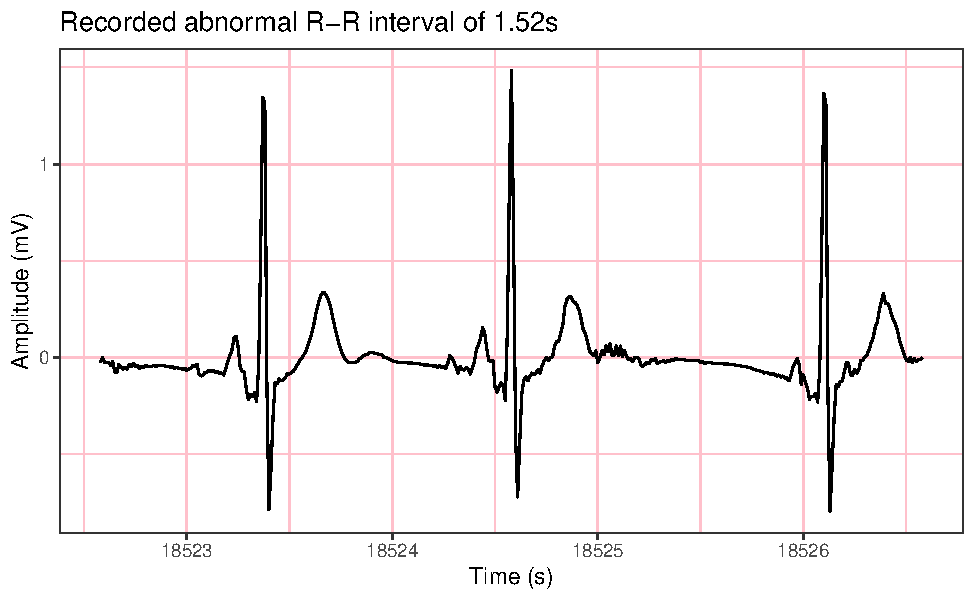
\includegraphics{report_files/figure-latex/abnormal-interval-32} \end{center}

\begin{center}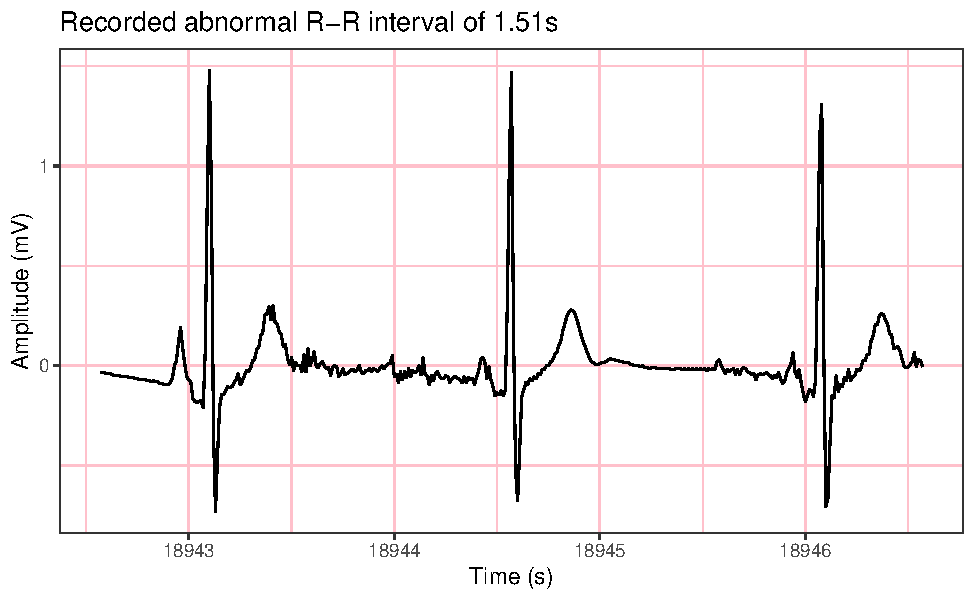
\includegraphics{report_files/figure-latex/abnormal-interval-33} \end{center}

\begin{center}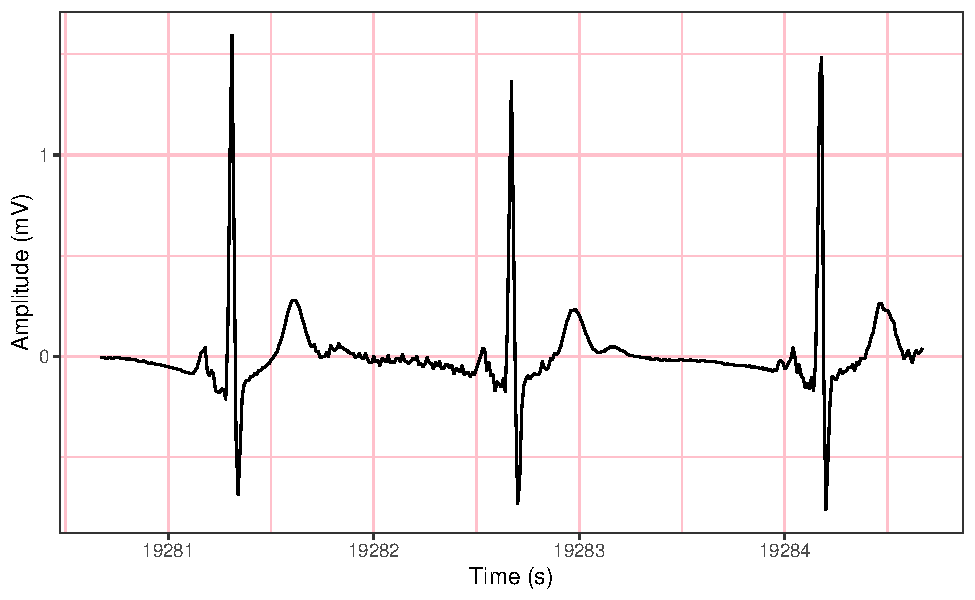
\includegraphics{report_files/figure-latex/abnormal-interval-34} \end{center}

\begin{center}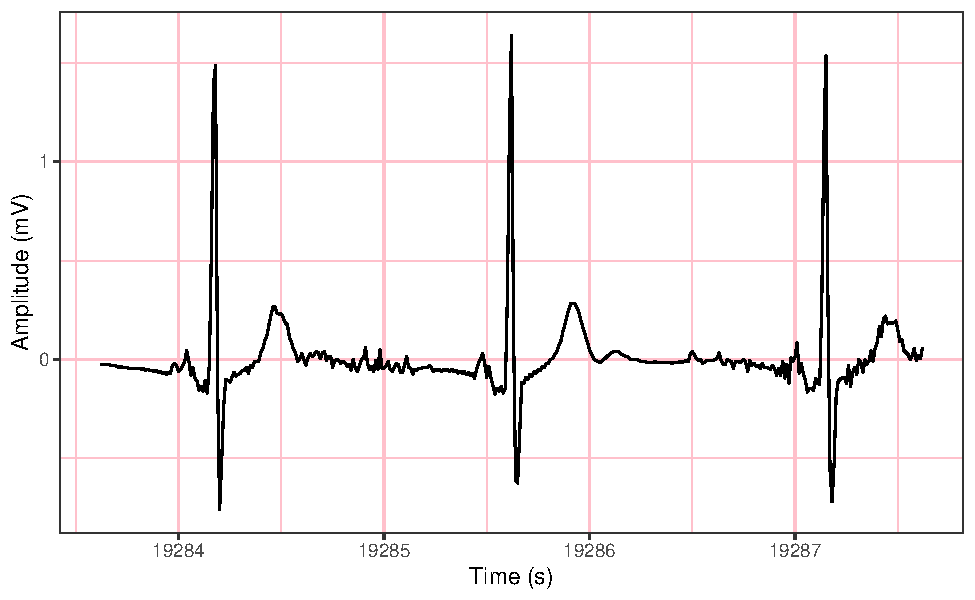
\includegraphics{report_files/figure-latex/abnormal-interval-35} \end{center}

\begin{center}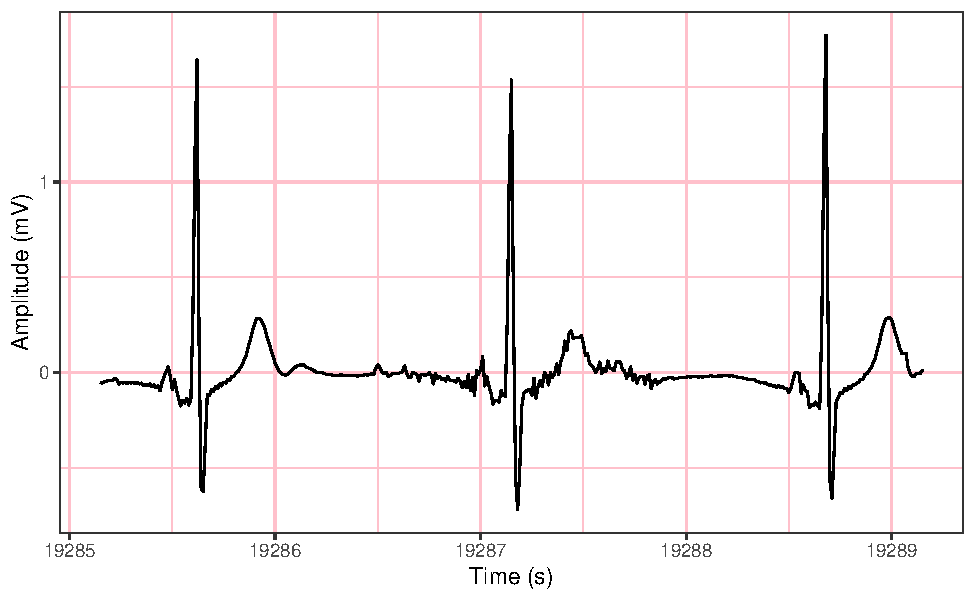
\includegraphics{report_files/figure-latex/abnormal-interval-36} \end{center}

\begin{center}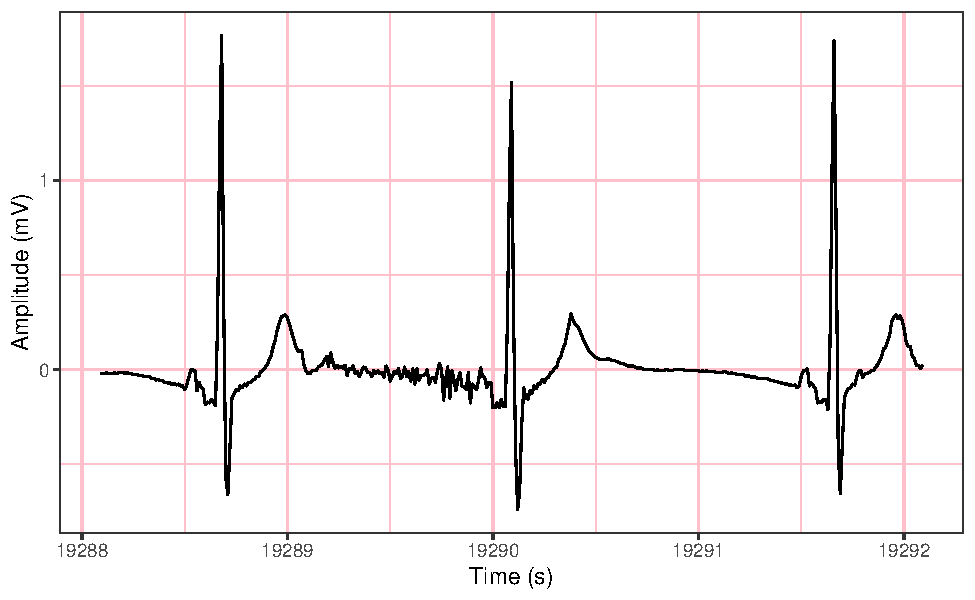
\includegraphics{report_files/figure-latex/abnormal-interval-37} \end{center}

\begin{center}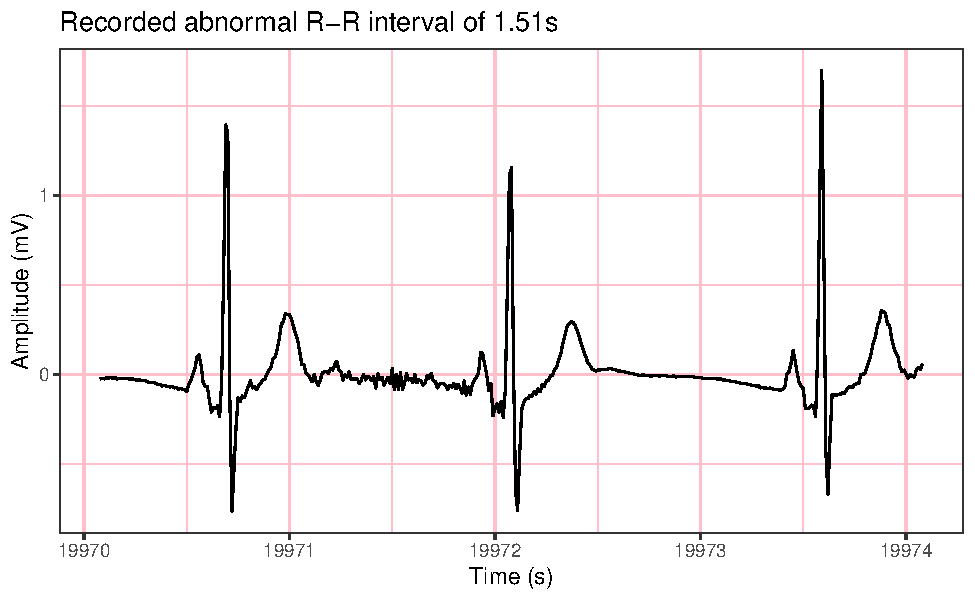
\includegraphics{report_files/figure-latex/abnormal-interval-38} \end{center}

\begin{center}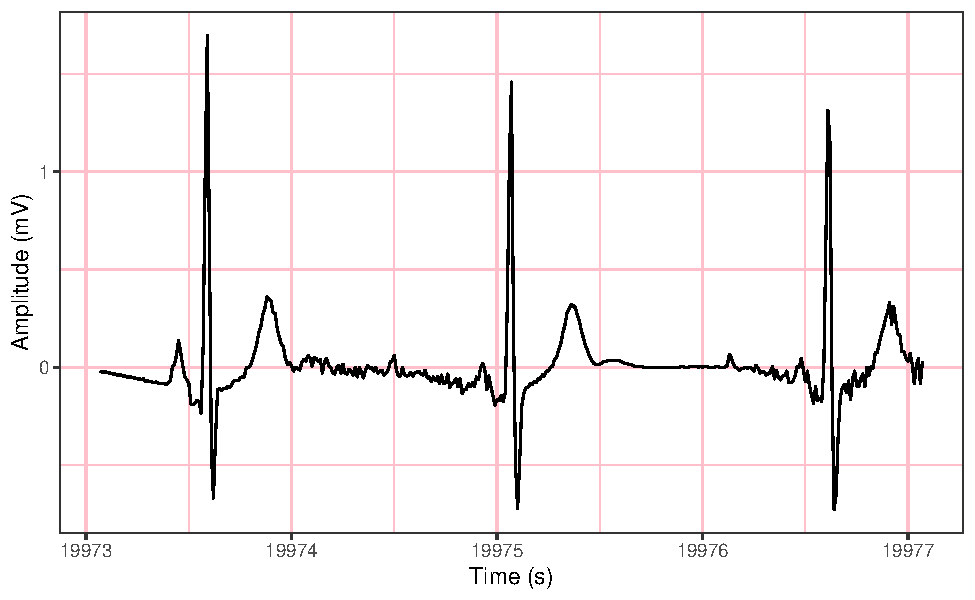
\includegraphics{report_files/figure-latex/abnormal-interval-39} \end{center}

\begin{center}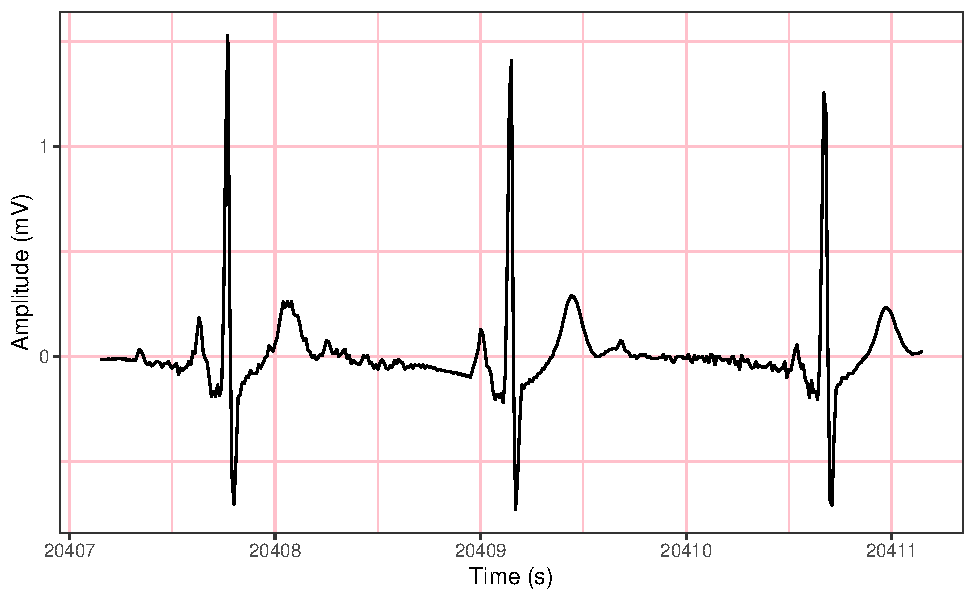
\includegraphics{report_files/figure-latex/abnormal-interval-40} \end{center}

\begin{center}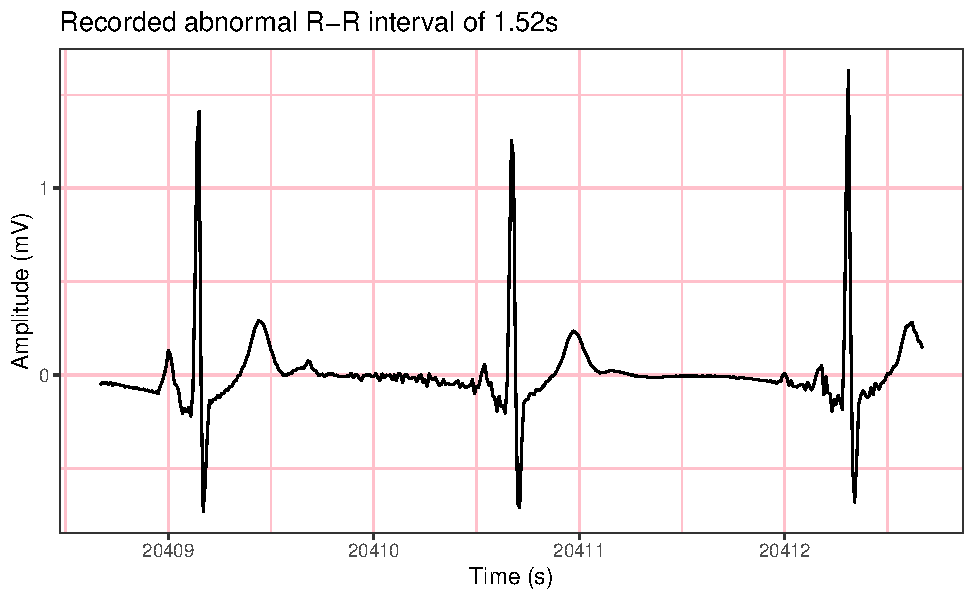
\includegraphics{report_files/figure-latex/abnormal-interval-41} \end{center}

\begin{center}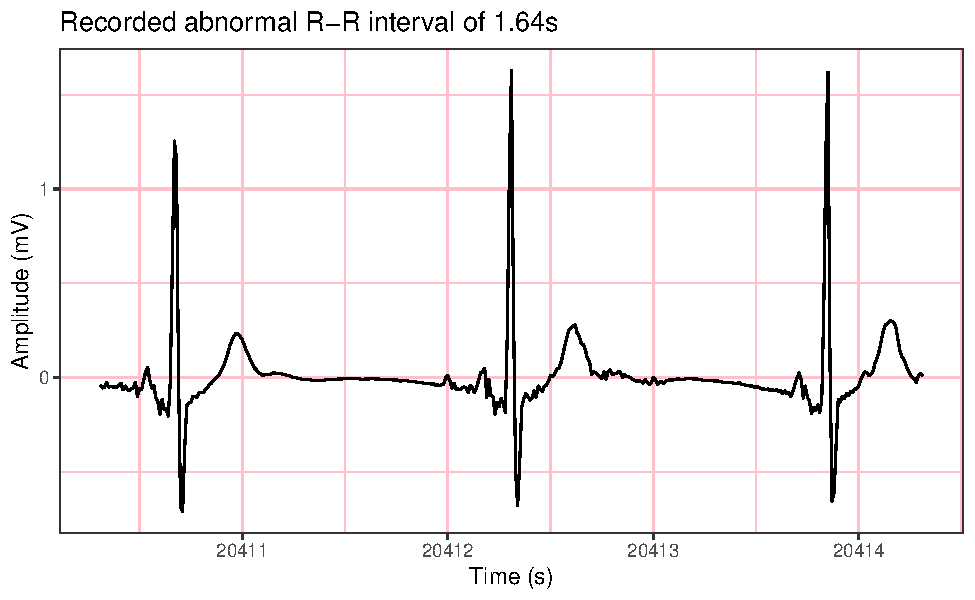
\includegraphics{report_files/figure-latex/abnormal-interval-42} \end{center}

\begin{center}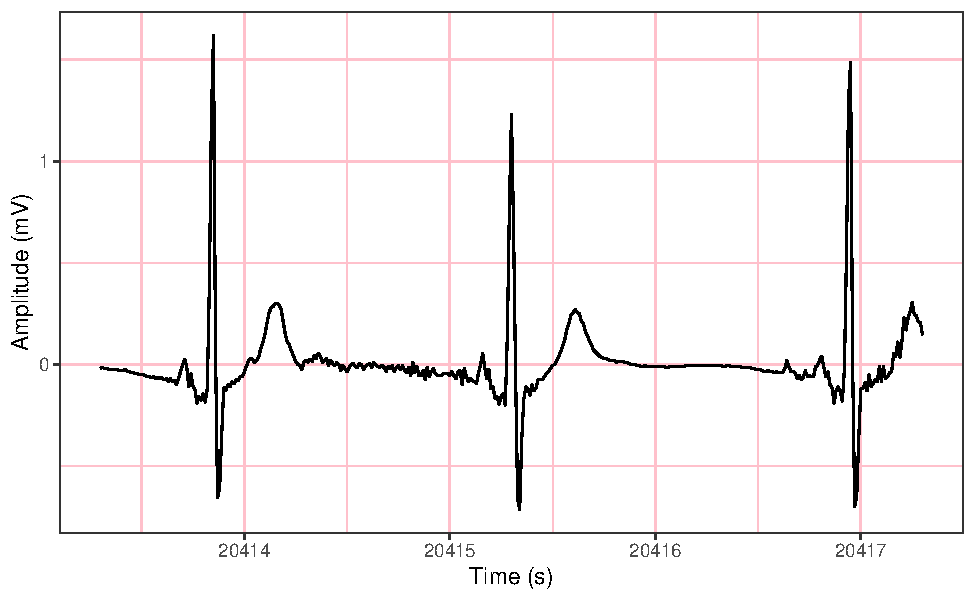
\includegraphics{report_files/figure-latex/abnormal-interval-43} \end{center}

\begin{center}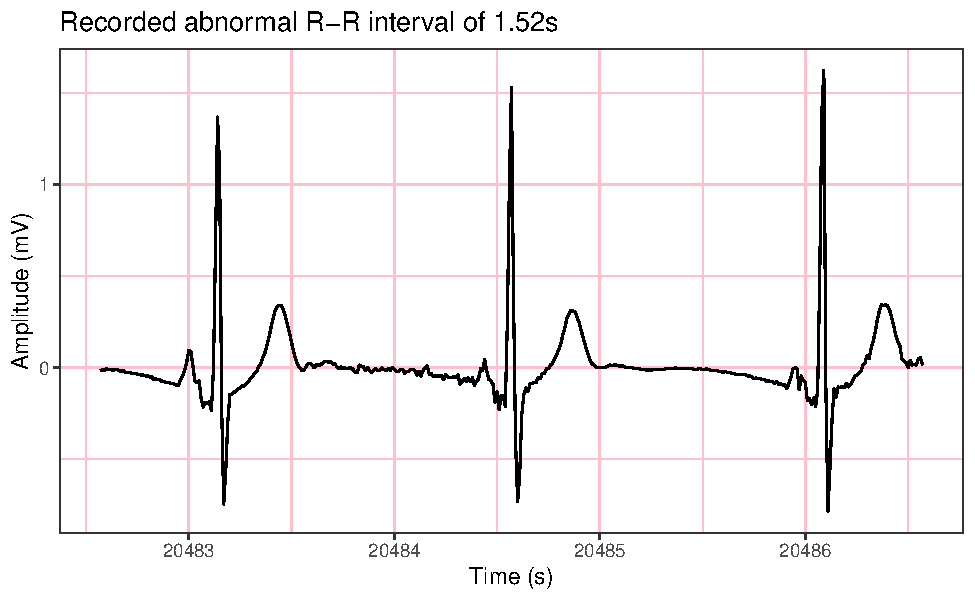
\includegraphics{report_files/figure-latex/abnormal-interval-44} \end{center}

\begin{center}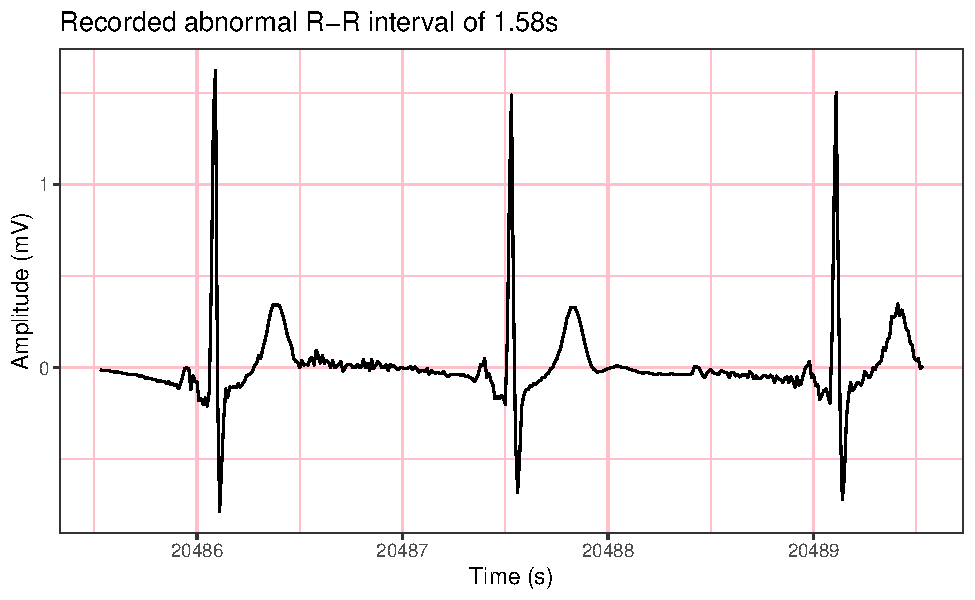
\includegraphics{report_files/figure-latex/abnormal-interval-45} \end{center}

\begin{center}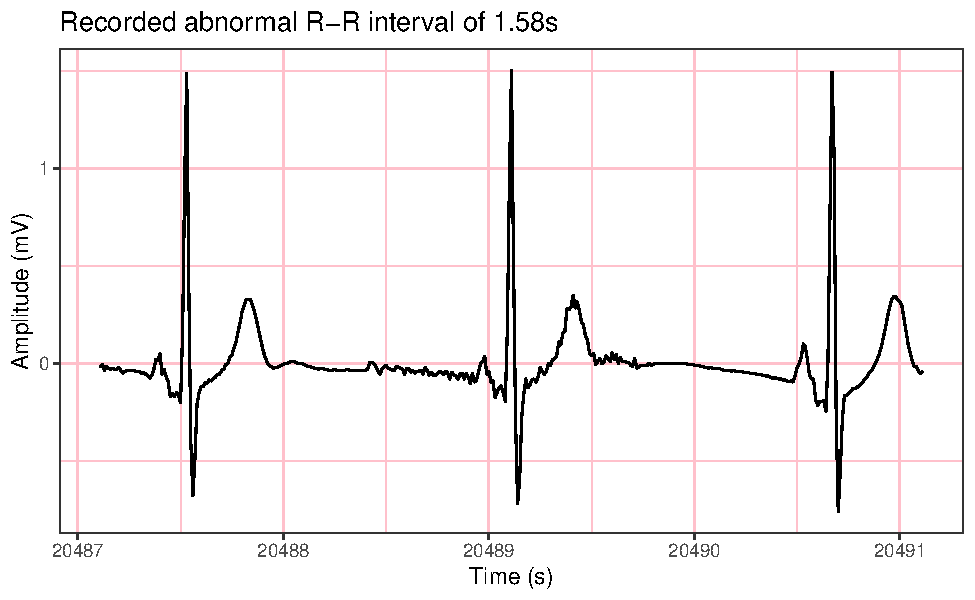
\includegraphics{report_files/figure-latex/abnormal-interval-46} \end{center}

\begin{center}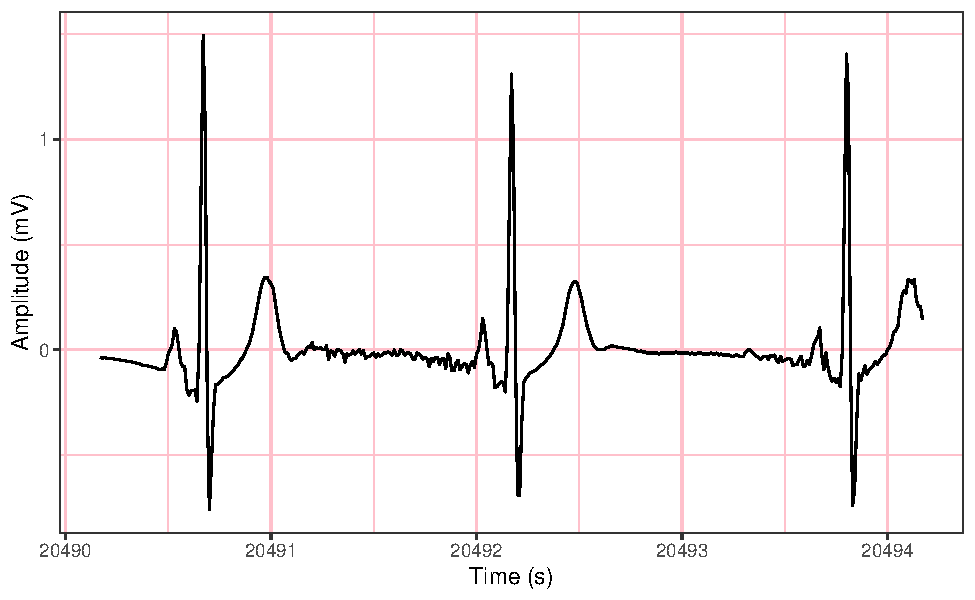
\includegraphics{report_files/figure-latex/abnormal-interval-47} \end{center}

\begin{center}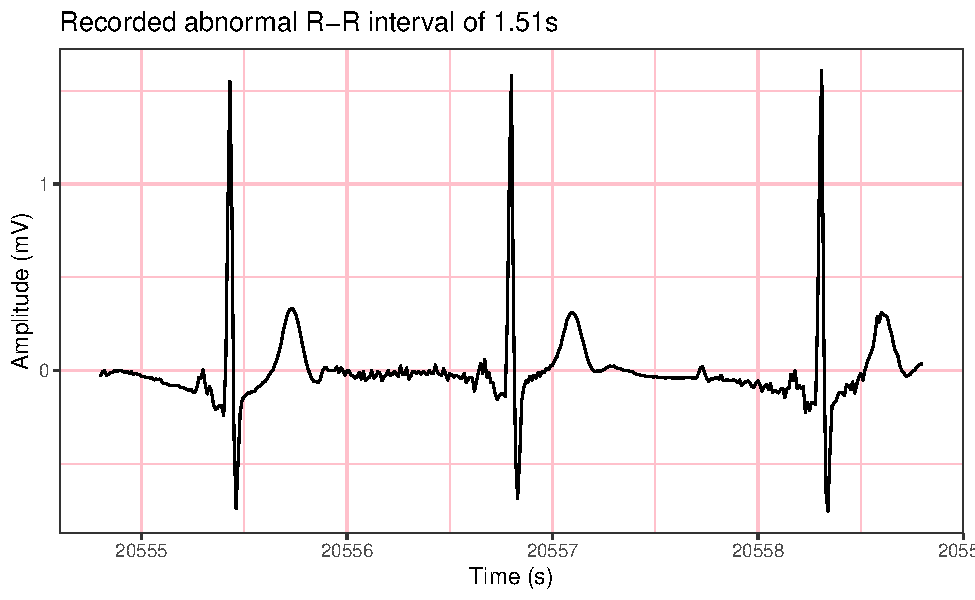
\includegraphics{report_files/figure-latex/abnormal-interval-48} \end{center}

\begin{center}\includegraphics{report_files/figure-latex/abnormal-interval-49} \end{center}

\begin{center}\includegraphics{report_files/figure-latex/abnormal-interval-50} \end{center}

\begin{center}\includegraphics{report_files/figure-latex/abnormal-interval-51} \end{center}

\begin{center}\includegraphics{report_files/figure-latex/abnormal-interval-52} \end{center}

\begin{center}\includegraphics{report_files/figure-latex/abnormal-interval-53} \end{center}

\begin{center}\includegraphics{report_files/figure-latex/abnormal-interval-54} \end{center}

\begin{center}\includegraphics{report_files/figure-latex/abnormal-interval-55} \end{center}

\begin{center}\includegraphics{report_files/figure-latex/abnormal-interval-56} \end{center}

\begin{center}\includegraphics{report_files/figure-latex/abnormal-interval-57} \end{center}

\begin{center}\includegraphics{report_files/figure-latex/abnormal-interval-58} \end{center}

\newpage

\hypertarget{references}{%
\section*{References}\label{references}}
\addcontentsline{toc}{section}{References}

\hypertarget{refs}{}
\begin{CSLReferences}{1}{1}
\leavevmode\vadjust pre{\hypertarget{ref-physiobank2000}{}}%
Goldberger, A. L., Amaral, L. A., Glass, L., Hausdorff, J. M., Ivanov,
P. C., Mark, R. G., Mietus, J. E., Moody, G. B., Peng, C.-K., \&
Stanley, H. E. (2000). Physiobank, physiotoolkit, and physionet.
\emph{Circulation}, \emph{101}(23), e215--e220.

\leavevmode\vadjust pre{\hypertarget{ref-apnea2000}{}}%
Penzel, T., Moody, G. B., Mark, R. G., Goldberger, A. L., \& Peter, J.
H. (2000). The apnea-ecg database. \emph{Computers in Cardiology 2000},
255--258.

\end{CSLReferences}

\end{document}
